% This is samplepaper.tex, a sample chapter demonstrating the
% LLNCS macro package for Springer Computer Science proceedings;
% Version 2.20 of 2017/10/04
%
\documentclass[runningheads]{llncs}
%
\usepackage{biblatex} %Imports biblatex package
% \usepackage[style=ieee,backend=biber,maxbibnames=99,block=space, sorting=none]{{biblatex}}
\addbibresource{ref.bib} %Import the bibliography file

\usepackage{pgf}
\usepackage{graphicx}

\usepackage{layouts}
% Used for displaying a sample figure. If possible, figure files should
% be included in EPS format.
%
% If you use the hyperref package, please uncomment the following line
% to display URLs in blue roman font according to Springer's eBook style:
% \renewcommand\UrlFont{\color{blue}\rmfamily}

\begin{document}
%
\title{MEP: A Comprehensive Medicines Extraction System on Prescriptions}
%
%\titlerunning{Abbreviated paper title}
% If the paper title is too long for the running head, you can set
% an abbreviated paper title here
%
\author{Ngoc-Thao Nguyen\inst{1,2}\orcidID{0000-0003-0252-6519} \and
    Duy Ha\inst{1,2}\orcidID{0000-0003-2077-0435} \and
	Khanh Tran\inst{1,2}\orcidID{0000-0002-0409-1304} \and
	Duc Nguyen\inst{1,2}\orcidID{0000-0002-2088-6000} \and
	Hieu Vo\inst{1,2}\orcidID{0000-0002-1260-021X} \and 
	Thanh Le\inst{1, 2}\orcidID{0000-0002-2180-4222}}
%
\authorrunning{Ngoc-Thao Nguyen et al.}
% First names are abbreviated in the running head.
% If there are more than two authors, 'et al.' is used.
%
\institute{Faculty of Information Technology, University of Science, Ho Chi Minh city, Vietnam \and
Vietnam National University, Ho Chi Minh city, Vietnam \\
\email{\{vohieu20122000, hvduy37, lankhanh1482, ducsinhvientinhnguyen\}@gmail.com}\\
% \email{18120018@student.hcmus.edu.vn} \\
\email{\{lnthanh, nnthao\}@fit.hcmus.edu.vn}}
\maketitle
%
  % typeset the header of the contribution
\begin{abstract}
Identifying drug names from prescription images has played an important role in the processing and storing of patient medical information. Based on our previous approach, we propose a new version named Medicines Extraction on Prescription (MEP) to recognize and extract proprietary medicines from prescription images obtained by smartphones. The proposed work employs some heuristic rules and a Temporal Convolutional Network model to extract pharmaceutical terms and classify them into drug names and active ingredients in OCR result texts. Experimentally, our model demonstrates the ability to recognize the names of drugs in the input image in a relatively short time, achieving a precision score of up to 0.94 on our datasets.


%However, the system has a limitation that the rate of drug omits still exists. This is the future challenge for the development team.
% In addition, a dataset of prescription images collected by our team is introduced. It is considered as a measure of the accuracy and uptime of the text recognition and detection system in prescriptions.

\keywords{Prescription Recognition \and Optical Character Recognition \and Medicines Classification \and Fuzzy Matching}
\end{abstract}
%
%
%
\section{Introduction}
Prescriptions are common for individuals and organizations involved in the medical field, especially patients. It contains a lot of critical information, including the patient's identity, the doctor's name, the name of the disease, the current condition and most importantly, the name of the medicine and the dosage used. Despite the details, the prescription does not clearly explain the origin, ingredients, and side effects that the drug brings to the user. This has led to an increase in the number of patients poisoning or, most seriously, death (due to side effects or allergies to some drug ingredients). In certain circumstances, improper medication usage might exacerbate chronic conditions. Furthermore, certain medicines may have major side effects on the body's organs. Depending on the drug administered, the body might heal or suffer long-term physical damage. The heart, liver, and kidneys are organ systems that are extremely vulnerable to harm.

According to statistics, from 1968 to 2019 in the US, 1,015,060 people died from a drug overdose. In addition, according to federal data released on November 17, the US recorded over 100,000 drug overdose deaths for the first time in the past 12 months, an increase of 28.5\% over the same period before \footnote{\url{https://edition.cnn.com/2021/11/17/health/drug-overdose-deaths-record-high/index.html}}.

% In addition, users may want to thoroughly lookup drug names on popular search engines such as Google, Bing. However, because prescriptions and drug names often contain quite specialized words, it inevitably causes specific difficulties and complications for users in the search process. There is a desire for a simple and easy-to-use system for looking up and identifying prescriptions, as well as a tool for managing drugs and the user's drug usage process.

For these mentioned reasons, a system for Medicines Extraction on Prescriptions (MEP) is introduced. Our user-friendly system has a low computational cost and fast processing time, making it widely-accepted by patients and medical facilities worldwide. Generally, MEP is a hybrid of recent popular approaches including OCR, Post-OCR, pattern matching, and natural language processing. This paper is organized as follows: problem statement is given in Section 1. Section 2 demonstrates the architecture of related techniques. Background technique and proposed recognition system are described in Sections 3 and Section 4, respectively. Experimental results on our datasets are presented in Section 5, and Section 6 provides conclusions and future work.


\section{Related work}
OCR functions as the major component of the prescription recognition system. The OCR operation usually consists of three main stages: text detection, text recognition, and drug name extraction. In this section, we briefly present each group's state-of-the-art algorithms and evaluate the method's appropriateness for our system.
\subsection{Text Detection and Recognition}

Text detection is the process of detecting and isolating text from the background of an image. Two typically used text detection methods are the traditional and deep learning methods. Traditional methods such as Scale Invariant Feature Transform (SIFT), Hough transforms, Features from Accelerated Segment Test (FAST) often extract text features manually. Therefore, this method is often complicated, quickly accumulates errors, and has many classification rules that must be manually optimized. With the evolution of deep neural networks in recent years, %deep learning models can yield superior results than traditional approaches in processing time and accuracy when trained with a good data set. 
several methods have utilized deep learning techniques, for instance, semantic segmentation and object detection in images. Semantic segmentation extracts blocks of text from a segmentation map created by the FCN and then creates a bounding box through post-processing. Some algorithms that employed this concept include TextSegNet, WordDetNet, and three CNN-based models DNet, SNet, CNet. 
%This approach can handle multi-oriented text, but individual text lines or words near each other need more postfix after the text spotting step. 
Another approach for text recognition in images takes inspiration from general object detection neural models, which are listed and examined in detail in this comprehensive survey \cite{ye2014text}. This method aims at recognizing the text in the scene, with its essence being to associate the texts as objects to predict the bounding box. 
%In addition, the direction will also be indicated to align the axis for the bounding box for multi-oriented texts.
Some generally used methods that leverage this approach are CTPN \cite{tian2016detecting}, CRAFT \cite{baek2019character}, EAST, SegLink.

Once the text is detected, the text recognition phase converts the recognized text into editable digital text. Recent text recognition methods can be classified into segmentation-based and segmentation-free. In a segmentation-based method, the text images are preprocessed and segmented before using a character classification model to recognize characters before aggregating them into lines. In contrast, the segmentation-free method recognizes the whole line of text at once by converting the text image into the output text string using the encoder-decoder framework.
%which consists of 4 stages. The first step is image preprocessing which removes background and image distortion using techniques such as spatial transformer network (STN), Thin-Plate Spline interpolation (TPS). The second step extracts features by mapping the input text image to a vector representing the features of the character, using methods such as HOG, VGGNet, ResNet. Subsequently, the context information contained in the text string is spotted and modelized using models like BiLSTM, deep one-dimensional CNN, CNN with receptive field correction. The last step predicts the output editable texts using Connectionist Temporal Classification Loss (CTC Loss), or attention mechanism. 
Some crucial techniques for text recognition include CRF (Conditional Random Field), CRNN (Regressive Convolutional Network), ASTER(Contextual Text Recognition Network).

\subsection{Post-OCR}
The text generated from the OCR step include all the content in the prescription. Recently widely used Post-OCR methods have been examined in great detail in this survey \cite{nguyen2021survey}. Since drug names are scientific, context-independent, and sentence-order insignificant terms, a dictionary of related terms is indispensable to extract drug names from the OCR text. 

Karthikeyan et al.\cite{karthikeyan2021ocr}  proposed an OCR post-processing method on medical documents employing a pre-trained model in natural language processing and a deep neural network model RoBERTa. The authors first used the Tesseract OCR tool to extract the text. In the post-processing step, biomedical entities were dismissed using Named Entity Recognition (NER) of the ScispaCy model, which belongs to Natural Language Processing fields. After withdrawing specific entities, the model detects error words and non-vocabulary words using spell checkers. RoBERTA is then employed to choose the most similar candidates to the error words. Considerable similarities between this method and the method of Thompson et al. \cite{thompson2015customised} are using spell checkers to identify error words. The most significant difference is Thompson added medical terms to spell checkers, while Karthikeyan takes advantage of the extensive medical terminology. However, the data set used is UK NHS, which is a private datasets containing patient private information. According to the authors, the method achieves 81\% accuracy without further training on the new datasets. The common feature of the models in these papers \cite{thompson2015customised, schulz2017multi, qader2019diagnosis, karthikeyan2021ocr} is that they are all to solve problems in a particular domain, including biomedicine and literature. Among them, Karthikeyan et al. proposed a post-processing approach using models in natural language processing. The Scispacy model used in this work \cite{karthikeyan2021ocr} could identify medical entities using Rxnorm, a database containing the active ingredients of drugs authorized for circulation in the United States. However, there was a distinction between the drug name and its active ingredient in the prescription we collected. While the drug name is the term given by the company that manufactured the drug, the active ingredient is usually the name of the chemical compound. Our proposed method partially solves this problem by creating a database containing drug names and their chemical compounds.

Our previous work \cite{nguyen2021developing} presented a prescription recognition model based on CRAFT and Tesseract OCR tool. We used fuzzy search based on Levenshtein distance to search for drug names in the database collected from Drugbank Vietnam \cite{drugbank}. However, the remaining issues in this system are the slow speed of drug extraction and the small size of the database. In addition, redundant information such as dosage used, name of the disease often causes noise and affects the speed and accuracy of the system. Therefore, in this paper, we continue to propose an improved model. Specifically, we redesigned the system, changing the models in stages and focusing more on the post-OCR step to increase the model's performance.

\section{Background}
\subsection{CRAFT}

% First of all, to get information for the drug identification system,  the problem of text recognition must be solved. Deep learning-based text recognition models excel in this step from reality. Initially, the researchers utilize CNN to find out which pixels belonged to text characters. Then, the text is considered as a special object, and neural networks are applied to encode the input image into feature maps. These feature maps are then fed into a classifier to predict and locate text areas. Recently, the CTPN structure is proposed and it consists of three main steps: fine-scale proposals for text detection, repeated linking text proposals and side-refinement. Fig.~\ref{fig_ctpn} illustrates these steps.

% \begin{figure}
% 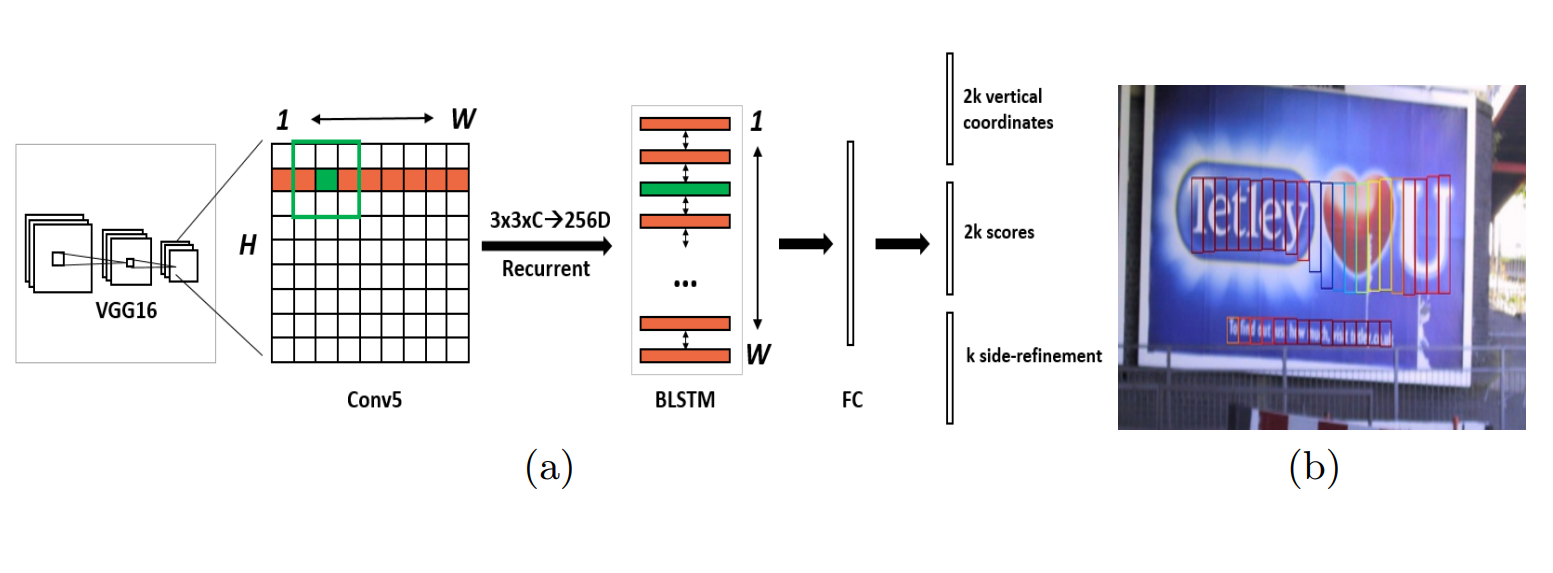
\includegraphics[width=\textwidth]{background/CTPN.png}
% \caption{The architecture of CTPN, adopted from \cite{tian2016detecting}}\label{fig_ctpn}
% \end{figure}

% In Fig.~\ref{fig_ctpn}, for text detection, the author first uses a VGG16 to extract features. Next, a sliding window slides through each location on the feature map of the final convolutional layer. Each position in the feature maps represents an attribute in the corresponding text area, which would create a "predict" that carries coordinate information and is labeled text/non-text. In fact, character detection could happen that the bounding box does not cover the entire text area because the character image has small, thin strokes or spaces between large letters. CTPN proposed a series of “fine-scale text proposals as a remedy for this problem. It is defined as a  sequence of small pieces of text that each contain one or more lines of text. An RNN layer is applied to encode this information. The results from the “predicts” would be fed into a BiLSTM network and then connected to a fully-connected layer. Integrating RNN significantly reduces false detection and obtains many text suggestions that were missed in the previous step simultaneously.  However, with the orientation-horizontal document, if the image is divided into proposals with a width of 16 pixels, it could lead to inaccurate localization or missing text areas. To further solve the outstanding problem, CTPN proceeds to estimate an additional part of the proposal on both the left and right sides (side-refinement step).


% To get information for the drug identification system, the problem of text recognition must be solved. Deep learning-based text recognition models excel in this step from reality. CRAFT is one of the most popular models used for regional text broadcasting. It detects each character area and the relationship among them. CRAFT predicts 2 metrics for each character bounding cell: (i) the region score is the probability that a given pixel is the center of the character, (ii) the affine score represents the center probability of the space among characters adjacent characters, which could be regarded as the extent to which characters are merged into one word \cite{baek2019character}. First, CRAFT generates the ground truths which are bounding boxes carrying information about the pointers and combines to give the bounds of each word. Instead of using map segmentation binaries to label each pixel individually, the author determines the encoding scale of the character center using a Gaussian heatmap. The procedure for representing the labels is as follows: 1) Prepare a 2-dimensional isotropic Gaussian map, 2) Do the computational transformation between the map and one by one character box, 3) Pack the Gaussian map into the area box. Next, with supervised learning, the characters found are broken down into small individual character sets for recognition. The images at the word level are cropped from the original image. The computational partitioning system calculates the affinity score for each region then applies an algorithm to split the characters region, thus creating bounding boxes at the character level. Eventually, it is based on the coordinates to return the character's barrier box to the origin.  Fig.1 is an illustration of CRAFT's X implementation.

To get information for the drug identification system, the problem of text recognition must be solved. In the deep learning era, CRAFT is one of the most popular models used for regional text broadcasting. It detects each character area and the relationship among them. CRAFT predicts 2 metrics for each character bounding cell: (i) the region score is the probability that a given pixel is the center of the character, (ii) the affine score represents the center probability of the space among characters adjacent characters, which could be regarded as the extent to which characters are merged into one word \cite{baek2019character}. 
\begin{figure}
\centering
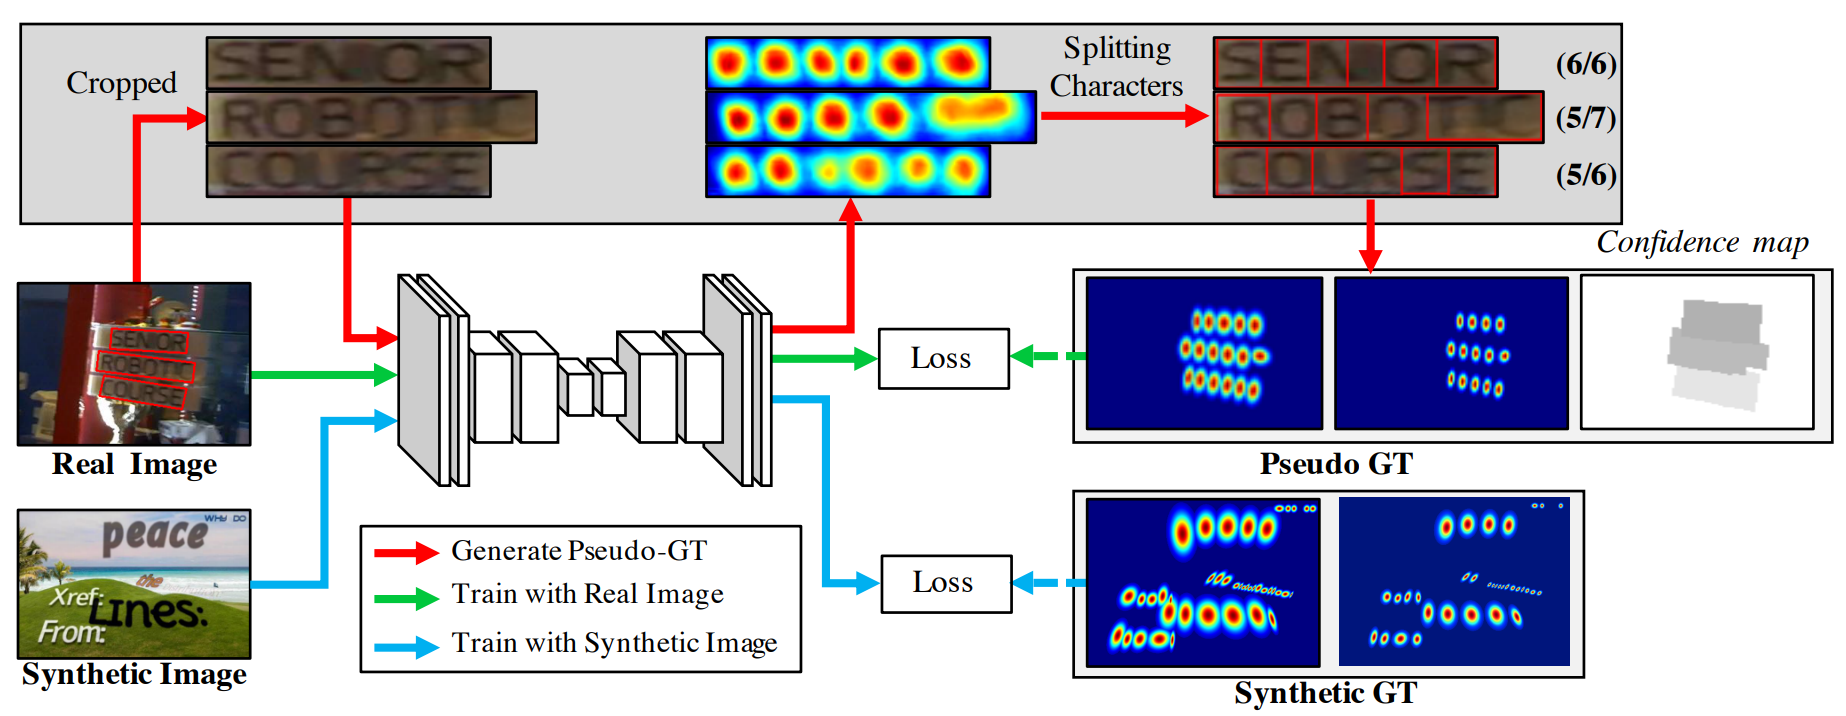
\includegraphics[width=0.7\textwidth]{background/CRAFT.png}
\caption{The architecture of CRAFT, adopted from \cite{baek2019character}}\label{fig_craft}
\end{figure}
The procedure for representing the labels is as follows. First, CRAFT generates the ground truths which are bounding boxes carrying information about the pointers and combines to give the bounds of each word. Instead of using map segmentation binaries to label each pixel individually, the author determines the encoding scale of the character center using a Gaussian heatmap. Second, with supervised learning, the characters found are broken down into small individual character sets for recognition. The images at the word level are cropped from the original image. The computational partitioning system calculates the affinity score for each region then applies an algorithm to split the characters region, thus creating bounding boxes at the character level. Eventually, it is based on the coordinates to return the character's barrier box to the origin.  Fig.1 is an illustration of CRAFT's implementation.


% In general, CTPN is capable of detecting text even in very blurry or layout-diverse images. It detects an entire text line that helps maintain text coherence. It could also recognize multilingualism without any additional processing steps. However, for tilted and skewed input images, CTPN does not perform correctly. Meanwhile, CRAFT detects each character region and the relationship between the characters then aggregates them. Instead of a bounding box around a line of characters like CTPN, CRAFT creates a bounding box for each word. The tilt, deviation of the input image almost does not affect the recognition results. However, the speed of this model is slow and might not be able to recognize single standing digits. 

% Unlike CTPN, another text detection model, which does not perform correctly for tilted and skewed input images, CRAFT detects each character region and the relationship between the characters then aggregates them that allows the tilt, deviation of the input image almost not to affect the recognition results.

% \subsection{Language model with OCR}

% Recently, many methods have been proposed to improve the accuracy of text recognition. One of them is trying to apply language models in the field of natural language processing to optical character recognition systems. In the VietOCR model, the author integrates the recognition model and the language model to produce positive results compared to traditional methods. Specifically, this model combines CNN with popular models in natural language processing such as Attention Seq2Seq, Transformer.

% In the model associated with Attention Seq2Seq---Attention OCR, since the LSTM model takes as input a 2-dimensional matrix, the feature map resulting from the CNN would be flattened before converting to the LSTM for prediction. As for the Transformer---Transformers OCR combination model, it has two principal parts Encoder and Decoder. It solves the outstanding problems of traditional technologies such as long processing time, poor concentration thanks to two special structures Multi-head attention and Positional encoding. Similar to Attention OCR, feature maps also need to be flattened before being put into position encoding. To optimize the model, VietOCR uses cross-entropy loss.

% According to the author, the accuracy of the model is stable and high even on the new data set. Using the Transformer model takes longer to execute, while its accuracy yields a negligible difference compared to another model. Seq2Seq is also more commonly used in many practical applications. In addition, VietOCR also allows retraining with new data, so this is an advantage for application developers.

\subsection{TCN}

To determine which texts are medicine in the database, we can use the Text Classification method. Convolutional Neural Network (CNN) architecture models can guarantee classification accuracy on simple strings. However, It goes terrible when texts have huge features or semantic ambiguous. To resolve, models that use Recurrent Neural Network (RNN) architecture were proposed. These models can retrieve the hidden features in sequence, which helps the model get the context in texts, like how the human brain work, making better accuracy.

Nevertheless, one drawback of RNN is the cost when dealing with extensive data. Shaojie Bai et al. \cite{bai2018empirical} proposed a new method called Temporal Convolutional Network (TCN) which is a compact version based on CNN architecture. In general, TCN stack with outstanding causal convolutions: dilated convolutions, which make TCN could learn pieces of information appeared in the past of the sequence effectively. Each output \(\textbf{y}_t\) depends on a series of \(\textbf{x}\) input, which is filtered by a parameter called \emph{filter size} on range \emph{\{0, 1, 2, …, t\}}. By measuring two-parameter \(d\) (dilation factor) and \(k\) (filter size), the model could control the suitable of deep in the sentence. With dilation, the operation of TCN brings breakthrough and recurrence similar to RNN. 
% Nevertheless, one drawback of RNN is the cost when dealing with extensive data. Shaojie Bai et al. \cite{bai2018empirical} proposed a new method called Temporal Convolutional Network (TCN) which is a compact version based on CNN architecture. In general, TCN stack with outstanding causal convolutions: dilated convolutions, which make TCN could learn pieces of information appeared in the past of the sequence effectively. Each output \(\textbf{y}_t\) depends on a series of \(\textbf{x}\) input, which is filtered by a parameter called \emph{filter size} on range \emph{\{0, 1, 2, …, t\}}. By measuring two-parameter \(d\) (dilation factor) and \(k\) (filter size), the model could control the suitable of deep in the sentence. With dilation, the operation of TCN brings breakthrough and recurrence similar to RNN. Fig.~\ref{fig_dilated} describes the architecture of the TCN model.

% \begin{figure}
% \centering
% 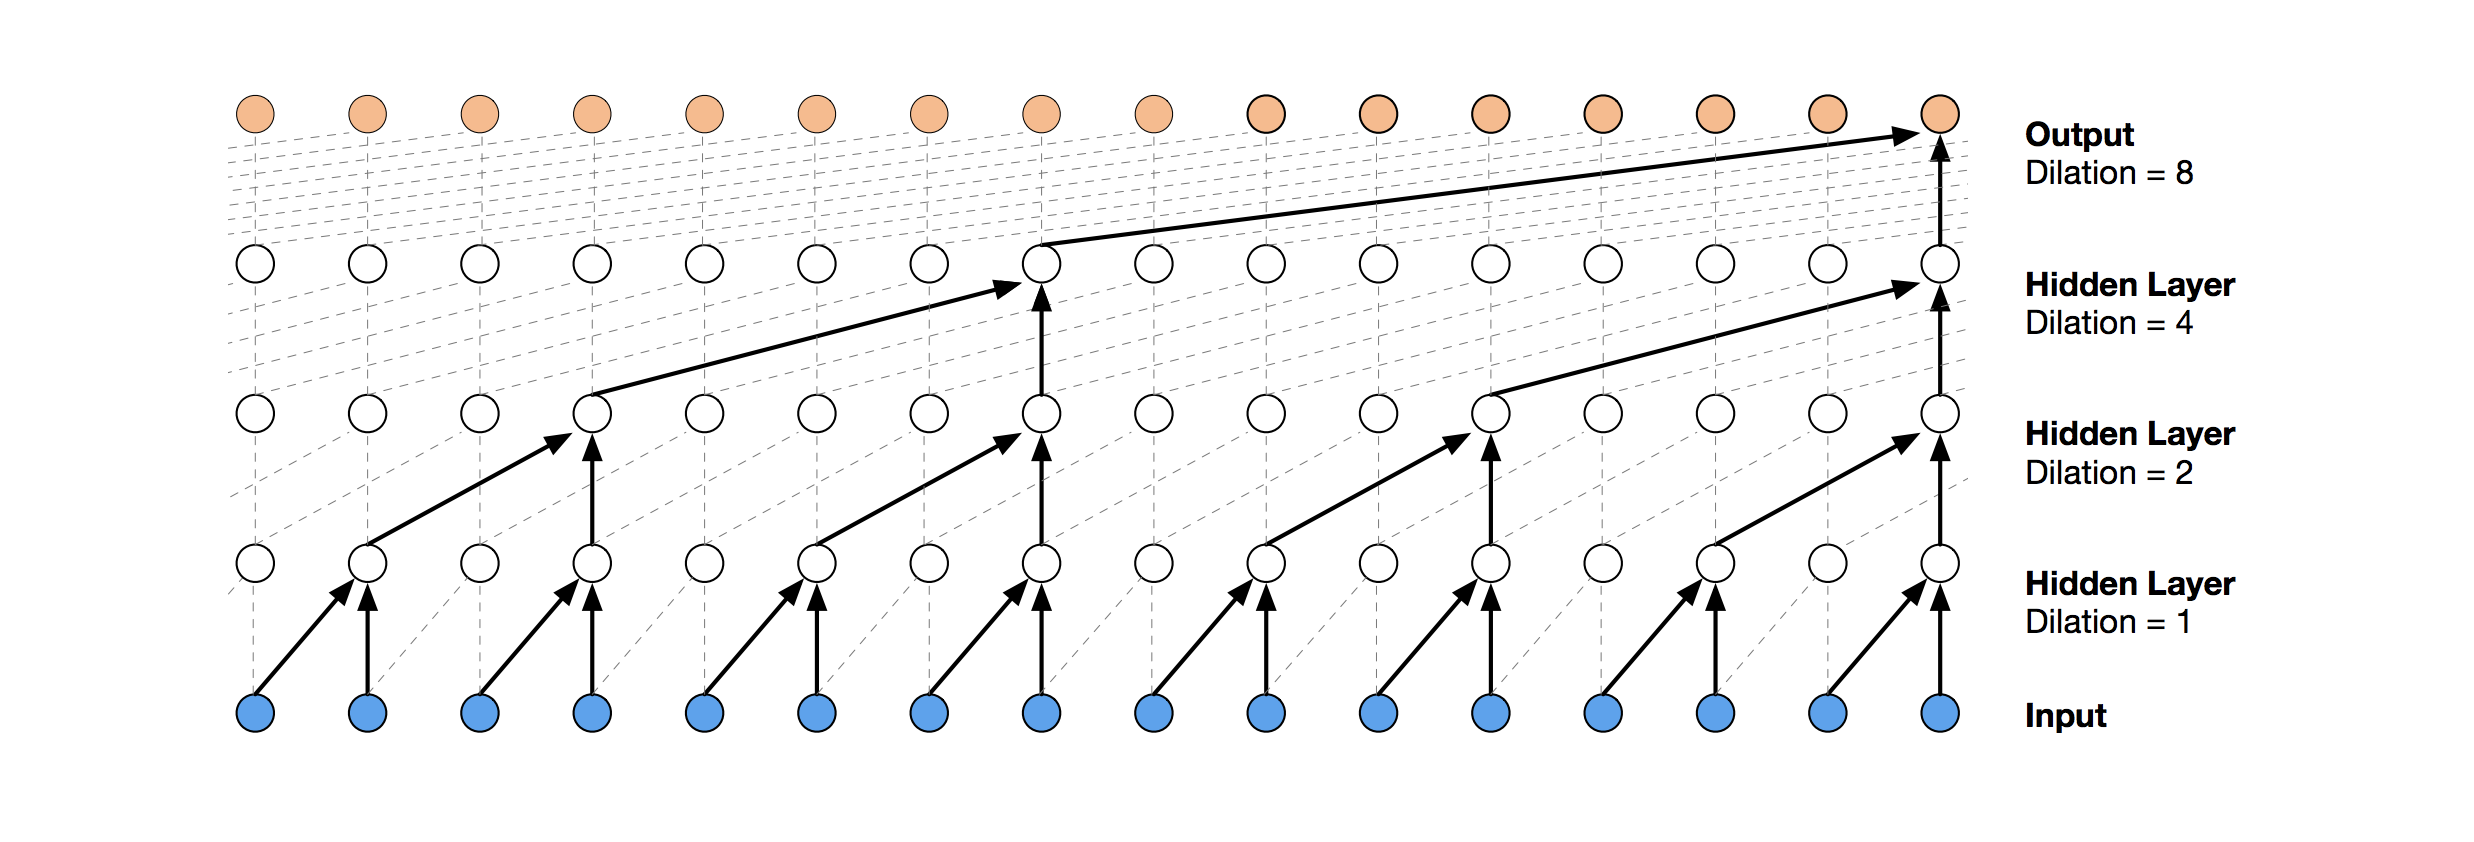
\includegraphics[width=0.8\textwidth]{background/Dilated_Conv.png}
% \caption{The architecture of TCN, adopted from \cite{TCN_architecture}}
% \label{fig_dilated}
% \end{figure}

In prescription recognition, medicine names have to be classified, which could have a unique characteristic in medical, different from other standard texts. Thus, TCN can be applied in the problem of drug name recognition and is mentioned in the proposed method section.

\section{A proposed system}
\begin{figure}
\centering
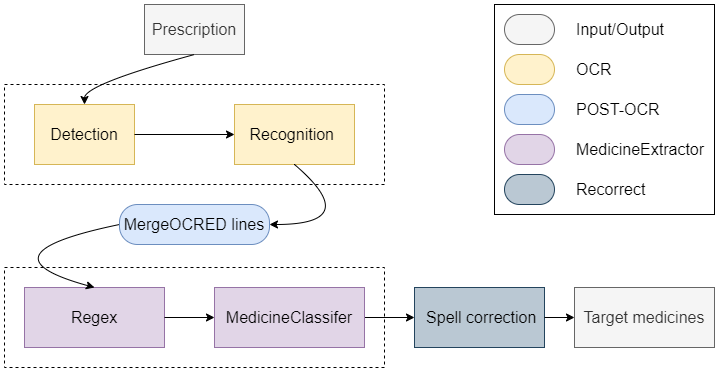
\includegraphics[width=0.7\textwidth]{method/proposed_method.png}
\caption{The architecture of Medicines Extraction on Prescription (MEP) system}\label{fig_proposed}
\end{figure}

Fig.3 exhibits the drug name recognition system MEP. It takes as input a prescription picture and feeds it into the detection model to detect the text region in the prescription. As stated, CRAFT generates a word-by-word bounding box that aids in the preservation of the precise medicine name as well as the tilt and skew of the input image, almost without affecting the recognition results. Therefore, CRAFT is well suited to the task of recognizing text in prescriptions. To recognize the detected text, the detection output is supplied into the recognition model. VietOCR is used in the text recognition stage due to its minimal complexity, high accuracy, and faster processing time than current popular models such as Tesseract. To keep the medicine's text, various vital drug names extraction methods and post-OCR procedures such as regex and MergeOCRED lines are employed. The Medicine classifier, in conjunction with the Correction approach, would provide the precise name of the medicine in the prescription.
\subsection{Craft-text-detector}
Compared to CRAFT, CTPN detects an entire row of text, which helps to maintain their coherence and faster processing time. However, CTPN does not handle tilted and skewed images effectively. Therefore, in this paper, we use the craft-text-detector, a library released by Fatih Cagatay Akyon framework to detect the text area. Based on the bounding boxes surrounding the words obtained from the conventional CRAFT architecture, this library conducts to group words on the same line/region into an object by applying thresholds. It not only creates the same effect as using CTPN but also retains the advantages of CRAFT.
\subsection{VietOCR}
VietOCR is an open-source Vietnamese text recognition model for that can be used with both handwriting and print. It was first released in 2020 by Quoc Pham and has been continuously updated in the past time. In the two Seq2Seq and Transformer installation methods, we use the former because the detection time is faster and the accuracy is not significantly different from the latter. VietOCR gets high accuracy even on a new datasets. Currently, VietOCR only supports text recognition line by line. Therefore when we have an image with many lines, we need to use supporting techniques to split the text into multiple lines first. This work we did in the craft-text-detector step. Specifically, the original image is divided into smaller images, containing the detected text areas and then inserted into VietOCR to return the resulting string.

\subsection{Medicine extractor}
% The recognition results include the whole existing text extracted from the input prescription. Aside from the name of drugs, prescriptions also contain data, such as patient information, drug dispensing facility information, disease diagnosis, and drug dosage, which are not our concerns. Therefore, there is a need to separate the drug names lines from the OCR result.  
Prescriptions, like receipts, frequently share the same qualities. The information is often provided in a systematic or semi-structured manner. Drug names are frequently listed in a consistent order and with the same pattern. By using two fundamental regular expressions, we may ease the separation of medicine names from prescriptions: 

\begin{figure}
\centering
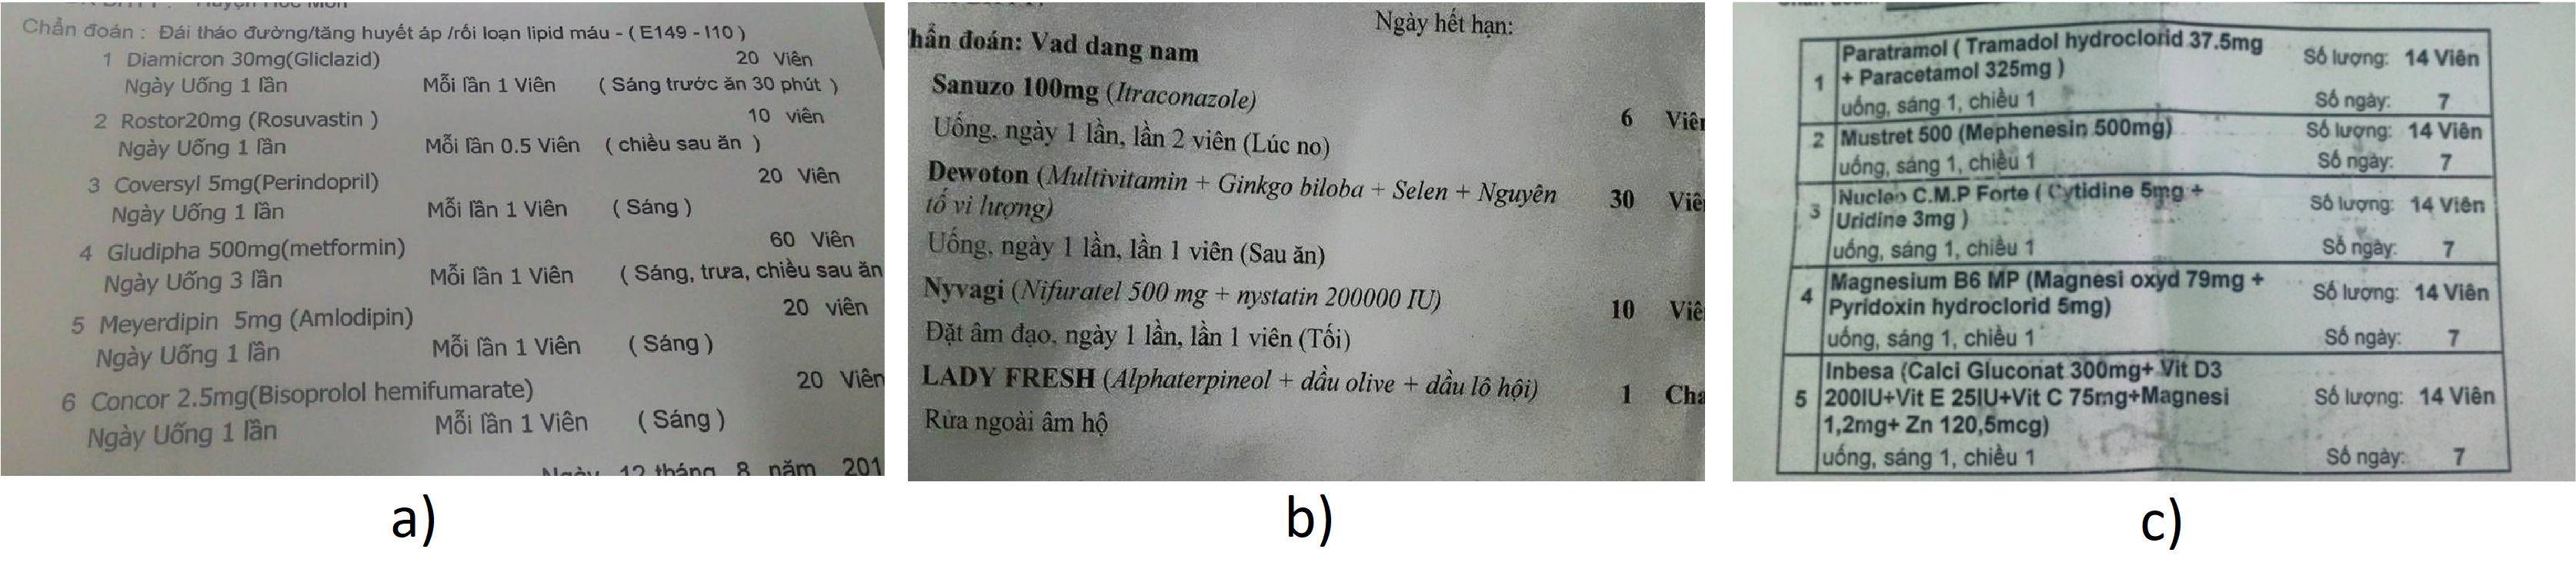
\includegraphics[width=0.8\textwidth]{method/regex_1_crop.png}
\caption{An example of prescription templates a) Medicine lines start with number, followed by medicine and ingredient b) Medicine lines start without number, followed by medicine and ingredient c) Prescription with medicine in multi-line} \label{fig_regex_1}
\end{figure}

\begin{itemize}
% \item[-] The drug names in a prescription are usually numbered. Each line starts with a number, followed by the drug name and possibly an additional active ingredient. This rule can extract the minimum of lines in the prescription and generate the highest probability of containing the drug name.

% \item[-] We modified the above rule for unnumbered prescription forms by defining the line containing the drug name that persisted according to the drug name structure followed by the active ingredient. Although this rule increases the number of lines that could be matched, it ensures the performance of the model, as well as a backup step if the OCR step cannot recognize the number before the drug name. 
\item[-] Lines containing a drug name often begin with a number, followed by a brand-name drug and possibly an active components. This rule can extract the minimum of lines in the prescription while increasing the likelihood of including the drug names.
\item[-] We extend the preceding rule for unnumbered prescription forms by specifying the line containing this structure. Although it increases the number of unrelated lines that may be matched, this technique assures the model's performance and serves as a backup step if the OCR step cannot recognize the number stand in front of the medicine name. 
\end{itemize}

Furthermore, some prescriptions include medicine names and active components spread across numerous lines. However, this is only a rare occurrence, so we do not handle it to avoid affecting the model's overall performance.
Fig.~\ref{fig_regex_1} shows examples of these format in prescription.  

After this phase, lines with a high likelihood of holding drug names would be extracted. In previous work, the entire output of the OCR matched the drug dictionary, causing the matching cost to grow as the size of the drug dictionary increased. To address this issue, the output of this step would be provided in medicine classifier Module.
\subsection{MergeOCR}
To ensure that regular expression in medicine extractor works correctly, lines containing drug names need to be bounded into boxes with all the necessary parts. However, if the image is fuzzy or noisy, the OCR process may not function properly. Rather of a single bounding box including all of digits, drug names, and drug ingredients, OCR generates numerous bounding boxes containing the separate components As a result, the extract medicine step may not work because it does not match the regular expression. Fig.~\ref{fig_merge} a) denotes a skewed text, one of the challenges of the OCR task
\begin{figure}
\centering
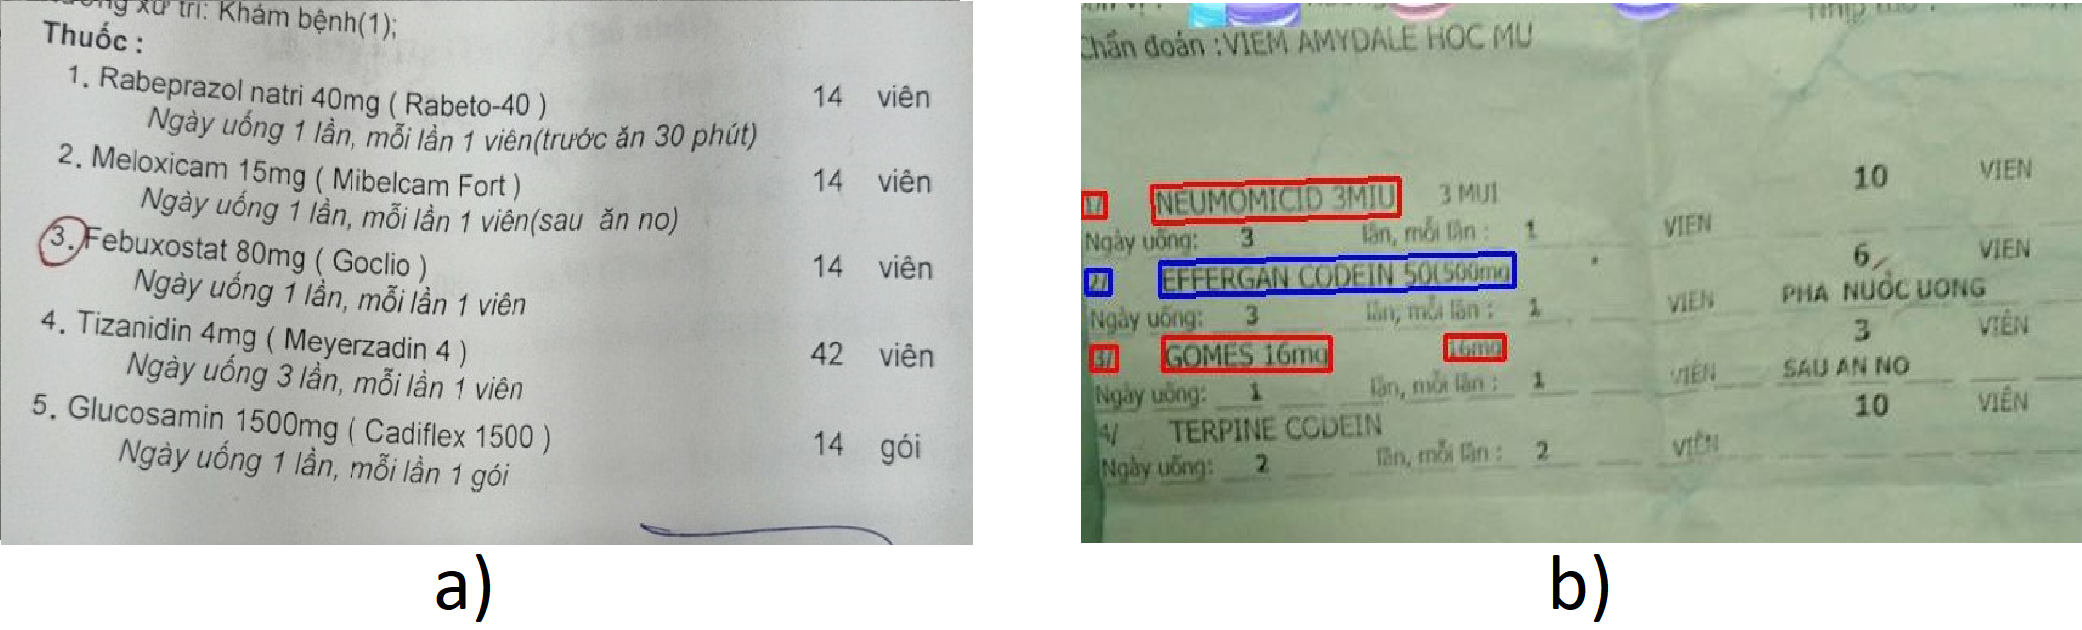
\includegraphics[width=0.9\textwidth]{method/merge_grouped.png}
\caption{a) An example show texts in prescription being skewed b) Result of MergeOCR, pieces of bounding box belong to a single line are merged correctly}
\label{fig_merge}
\end{figure}

To overcome this problem, an extended step named MergeOCR is recommended to group bounding boxes of texts belonging to the same line into a single line of text. % In addition to a line being split into different bounding boxes,  the boundaries among these bounding boxes could not be separated. Therefore, the proposed algorithm needs to overcome both these aspects effectively. Specifically, w
The AHC (Agglomerative Hierarchical Clustering) technique is used. The distance of the two bounding cells is calculated based on the y-axis coordinate distance on the 2D coordinate system. The principal advantage of AHC is that it is efficient and straightforward for this case. There is no need to predetermine the number of clusters, often referred as the number of lines in prescription. 
In this way, groups of words that are closest to each other could be prioritized and set thresholds to finish the merge process to optimize performance quickly. As merging OCR result texts is performed after the recognition step, the bounding boxes located on a line are still recognized separately, which makes VietOCR's recognition more effective and avoids interference. After the MergeOCR step, strings corresponding to the bounding box could join the correct x-axis order on the 2D coordinate system. %This line pooling makes much sense for the model before putting the data into the regex to extract the drug names. 
Fig.~\ref{fig_merge} b) shows the result of MergeOCR when grouping bounding boxes.
\subsection{Medicine Classifier}
\begin{figure}
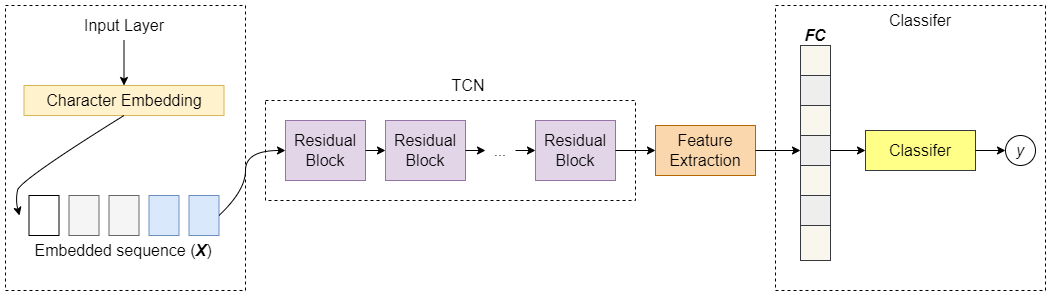
\includegraphics[width=\textwidth]{method/classifer_0.png}
\caption{Proposed medicine classifier architecture} \label{fig_class_0}
\end{figure}
After extracting lines containing drug names, the next task is to get the exact drug name in these lines. In particular, although most prescriptions have a fixed form with ordinal numbers, there is no common standard for the order between drug names and active ingredients. The drug name can precede the ingredients or vice versa, or even cases have no ingredients in that line. Therefore, the model needs to help classify a piece of text as a drug name or not, and simultaneously reduce the processing time of the entire output. %, and solve the problem more accurately. 
Based on the analyzed advantages of the TCN, it is used for this medicine classification model. Fig.~\ref{fig_class_0} shows the architecture of medicine classifier. 
The model structure includes two main parts, specifically as follows. In the first part, the input text would be pushed through the character embedding to convert to a sequence of characters. Then through padding with the longest sentence in the training phase, we represent different sentences of the same size. %Text classification is often applied to classify a whole sentence, paragraph, or essay. Therefore, people often use word embedding to help the model learn the text context better by the association among words. However,  it is short-text in medicine names. Only a few words are maximum. Drug names are often composed of several characters that are meaningless when put together, unlike the structure of ordinary words. Therefore, we propose using character embedding instead of word one. This way can both fix the problem and deal with misspelling medicine names. A long enough sequence for short-text could be obtained when using character embedding that limits overfitting. 
The second part is the TCN model, which aids to learn the features of the character embedding sequence. Because a missing or incorrect character has no effect on the overall strings, it is guaranteed to operate even if the drug names are misspelled. Furthermore, TCN's performance is extremely good. It can processing a large amount of data in a short period of time. TCN output is sent to fully connected layers, where it is classified into three categories: medicine names, active components, and others. 
% We collect data to train MedicineClassifier from drug dictionaries, which contain both medicine names and ingredients. For other classes, they are labeled as non-medicine or non-ingredient. All training data are filtered and cleaned to have the same min, max, mean and median features. Moreover, to ensure labels are in the short text, the number of words must be smaller than five
\subsection{Context-aware spell correction}
% After the MedicineClassifier step, many lines not containing the medicine names or ingredients were removed. The fewer lines are retained, the shorter the processing time is that optimizes the cost of the entire system. However, there is confusion between the drug name and the ingredient. 

\begin{figure}
\centering
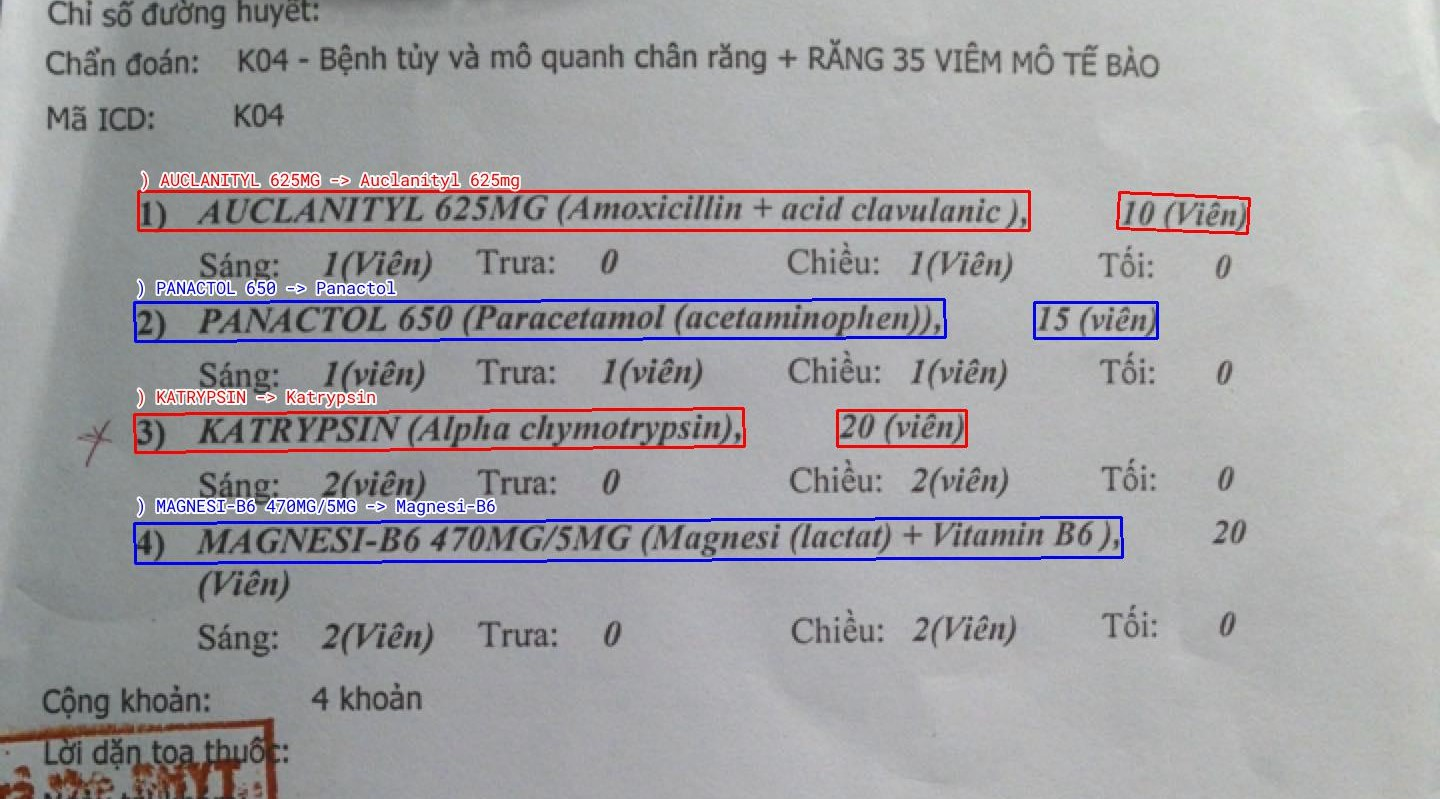
\includegraphics[width=0.7\textwidth]{method/fuzzy_0.jpg}
\caption{Corrected output of proposed Prescription Recognition system} \label{fig_fuzzy_0}
\end{figure}
A drug name sometimes could be also the ingredient and vice versa, but the medicine classifier model divided them into either drug names or ingredients. By using threshold, this last step filters the remaining lines to extract the most likely of being drug names by comparing each of them with a limited medicine names dictionary, then correcting them. This matching principle is based on edit distance, e.g. Levenshtein mentioned in previous work \cite{nguyen2021developing}, is the number of steps it takes to transform one string into another, used in many post-processing methods. 
Fig.~\ref{fig_fuzzy_0} shows our overall system's output applied spell correction.
% Sometimes, the drug name is both the ingredient and vice versa, but MedicineClassifier model divided them into either drug names or ingredients. Therefore, this last step filters the remaining lines to extract the most likely of being drug names by comparing each of them with a limited dictionary of drug names. If the match rate is higher than a threshold, it would be kept and corrected to the exact drug name in the dictionary. This matching principle is based on the edit distance, which is the number of steps it takes to transform one string into another. The smaller the number of steps, the more similar these two sequences are. Since our dictionary is a medical-specific lexicon collected from DrugBank Vietnam, the final results would be OCR error-free and only contain proper drug names. This way enhances the cost and accuracy of the system. For example, the word \emph{augmenta} has the same distance as \emph{augmentin} and \emph{augmented}. However, \emph{augmentin} would be chosen, as it is the accurate name of the medicine, while \emph{augmented} does not exist in the dictionary. 

% In previous work \cite{nguyen2021developing}, Levenshtein is mentioned as a metric for edit distance, used in many post-processing methods. The Levenshtein-based distance calculation method is leveraged to ensure the model's accuracy. However, there are some cases that both drug names and active ingredients match the dictionary. Unique drug names having the highest possibility of being medicines in the output of MedicineClassifier would be chosen. Fig.~\ref{fig_fuzzy_0} shows our overall system's output applied spell correction.


\section{Experiment}
\subsection{Datasets}
The datasets for model evaluation includes 1500 images with more than 10000 different drugs. Each drug name is surrounded by a bounding box labeled with the correct drug name. Original images in our datasets have been downloaded from a Facebook group called "KHO DON THUOC"\footnote[1]{https://www.facebook.com/groups/392636900896314}, a small group created to gather prescriptions from all over the world and collected manually from large and small hospitals in the area. The manual check is conducted to ensure there is no duplication. 

Although the primary language of this datasets is Vietnamese, drug names are often scientific names, so they are less affected by Vietnamese punctuation or grammar. This datasets contains prescription images captured with the phone's camera, brightness or tilt angle subject to change. Although these conditions are similar to reality, they unintentionally create a big challenge for recognition models: how to accurately identify text under challenging conditions of brightness and tilt angle. Therefore, this datasets measure the accuracy and uptime of the prescription text recognition and detection system.

% The dataset for model evaluation includes 1500 images with more than 10000 different drugs. Each drug name is surrounded by a bounding box labeled with the correct drug name. This data set is collected from hospitals and websites that specialize in drugs.

% Although the primary language of this dataset is Vietnamese, drug names are often scientific names, so they are less affected by Vietnamese punctuation or grammar. This dataset contains prescription images captured with the phone's camera, brightness or tilt angle subject to change. Although these conditions are similar to reality, they unintentionally create a big challenge for recognition models: how to accurately identify text under challenging conditions of brightness and tilt angle. Therefore, this dataset measure the accuracy and uptime of the prescription text recognition and detection system. In the following sections, we describe collecting and labeling this dataset.

% Images in our dataset have been downloaded from a Facebook group called "KHO DON THUOC", a small group created to gather prescriptions from all over the world and collected manually from large and small hospitals in the area. We have done the checks to ensure there is no duplication.

% Most of the images in our dataset have been downloaded from a Facebook group called "KHO DON THUOC", which is a small group created to gather prescriptions from all over the world. In addition, many prescriptions were collected by us from large and small hospitals in the area. We have done the checks manually to ensure there is no duplication. The final dataset contains 1008 images from the Internet and 492 images collected and taken by team members from the hospital.

%A few images taken perform the sample labeling process to estimate a suitable process for the dataset. The bounding box is drawn around the text that is the drug name. The bounding box's coordinates and drug names were saved in a semi-structured text file (JSON). After completing the testing phase on the initial images, statistical techniques are applied to evaluate the labeling results then give out judgments about the labeling results to update the labeling process to improve the quality and consensus in the labeling results.

\subsection{Parameter settings}

This section features parameters and hardware for the proposed system in the experiment. For text detection, we modified CRAFT parameters: \(text\_threshold = 0.7\) and \(link\_threshold = 0.4\). We config sequence model VietOCR in recognition step to \(vgg\_seq2seq\). The threshold of MergeOCR is at 0.016, which determines the sensitivity of the clustering process. In medicine classifier, we set padding size to 300, filter size \(k = 2\), dilation factor \(d = [1, 2, 4]\). The medicine classifier threshold to confirm whether the text could be medicine is set to 0.6. Finally, the threshold to confirm and correct medicines is 0.85.
% We experiment with the whole proposed system in the same machine hardware, which has two core CPU Intel Xenon @2.20GHz, GPU Tesla K80 controlled by CUDA Version 11.2. 

\subsection{Evaluation Metrics}

Precision and recall are the major measurements we employ in the experiment. To assess the model's accuracy, an extra H-mean metric is also utilized. 
\begin{equation} \label{eq_precision}
   Precision = \frac{|\{accurate\;drugs\}\:\cap\:\{retrieved\;drugs\}|}{|\{retrieved\;drugs\}|}
\end{equation}
\begin{equation} \label{eq_recall}
   Recall = \frac{|\{accurate\;drugs\}\:\cap\:\{retrieved\;drugs\}|}{|\{accurate\;drugs\}|}
\end{equation}
\begin{equation} \label{eq_hmean}
   H{\text -}mean = 2\;\frac{Precision\:\cdot\:Recall}{Precision\:+\:Recall}
\end{equation}
Equation (\ref{eq_precision}), (\ref{eq_recall}), and (\ref{eq_hmean}) show the definition of Precision, Recall and H-mean. These metrics are used in the overall of the proposed prescription recognition system.
% Precision denotes the proportion of properly predicted drug names in the total
% output given by the system, whereas Recall shows the right prediction rate for
% all drug names in the data set. From the above two metrics, H-mean is also
% computed to evaluate the model’s quality in general.
\subsection{Result}
% Table 1 shows the experimental results after applying the introduced method. After the post-processing stage, the model achieves Precision and Recall of 0.94 and 0.73 respectively that increase by 0.4 and 0.56 points sequentially when compared to the model introduced by Nguyen et al. \cite{nguyen2021developing}.
Table ~\ref{tab1} shows the experimental results of new method and our old system \cite{nguyen2021developing}. The proposed model identifies effectively drug names in the data set, which outperforms the previous version with Precision and Recall up to 0.94 and 0.73, which increase by 0.4 and 0.56 respectively. However, the Recall score is just 0.73. In general, the cause is that the input data contains several errors. Simultaneously, the value of these metrics is heavily reliant on the medicines extraction step. This could be improved in the future if appropriate heuristic rules are implemented to make drug name extraction more efficient.
% \usepackage{siunitx}

\begin{table}
\centering
\caption{Evaluation on previous and upgraded system}\label{tab1}
% \begin{tabular}{|S[table-format=15.0]|S[table-format=10.2]|S[table-format=7.2]|S[table-format=7.2]|}
\begin{tabular}{|c|ccc|}
\hline
Model           & @Precision & @Recall & @H-mean  \\ 
\hline
Method in \cite{nguyen2021developing}      & 0.54       & 0.17    & 0.26     \\ 
\hline
\textbf{MEP} & \textbf{0.94}       & \textbf{0.73}    & \textbf{0.82}     \\
\hline
\end{tabular}
\end{table}

\begin{table}
\centering
\caption{The importance of medicine extractor in Prescription Recognition system}\label{tab2}
% \begin{tabular}{|S[table-format=15.0]|S[table-format=10.2]|S[table-format=7.2]|S[table-format=7.2]|}
\begin{tabular}{|c|c|c|c|c|}
\hline
Model           & OCRed text & MedicineExtractor & Spell correction & Output \\ 
\hline
Method in \cite{nguyen2021developing}      & Allpovic & - & [Alpovic]@0.9 & Alpovic     \\ 
\textbf{MEP} & Allpovic & \textbf{Allpovic} & [Alpovic]@0.9 & Alpovic     \\
\hline
Method in \cite{nguyen2021developing}      & Eperison 50mg (Macnir) & - & [Macnir]@0.6 & -      \\ 
\textbf{MEP} & Eperison 50mg (Macnir) & \textbf{Macnir} & [Macnir]@1.0 & Macnir     \\
\hline
\textbf{MEP} & Diovan 160mg (Valsartan) & \textbf{Diovan 160mg} & [Diovan 160]@0.94 & Diovan 160     \\
\hline
\end{tabular}
\end{table}
In addition, table~\ref{tab2} demonstrates how MEP achieves more stable results than the method in \cite{nguyen2021developing}. With the first medicine's name "Alpovic", both MEP and system in \cite{nguyen2021developing} work efficiently with high result confidence even though the inputs are misspelled. But when the output text of the OCR task is "Eperison 50mg (Macnir)", the old method can not separate drug and ingredient completely before applying it to the spell correction stage. As a result, the confidence metric is only 0.6, less than the configured threshold, so the model marks this text as non-drug. MEP overcome this restriction by adding a new layer to extract exactly drug names from the OCR stage, thanks to Medicine Classifier. No matter the complexity of OCRed text lines, the proposed method always knows which one is the drug name. In table~\ref{tab2}, MEP smoothly extracts "Macnir" and "Diovan 160mg" and throws them to the spell correction stage, finally achieving clear outcomes with excellent confidence. 

\begin{figure}
\centering
% 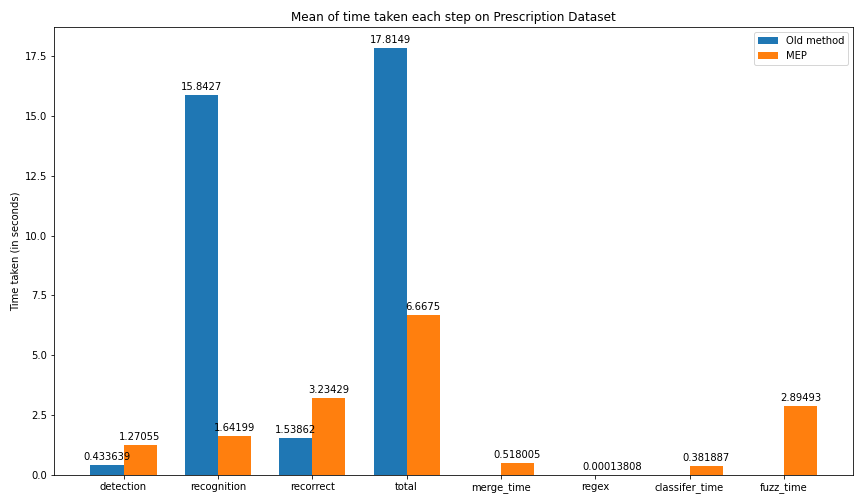
\includegraphics[width=0.7\textwidth]{experiment/barchart.png}
% 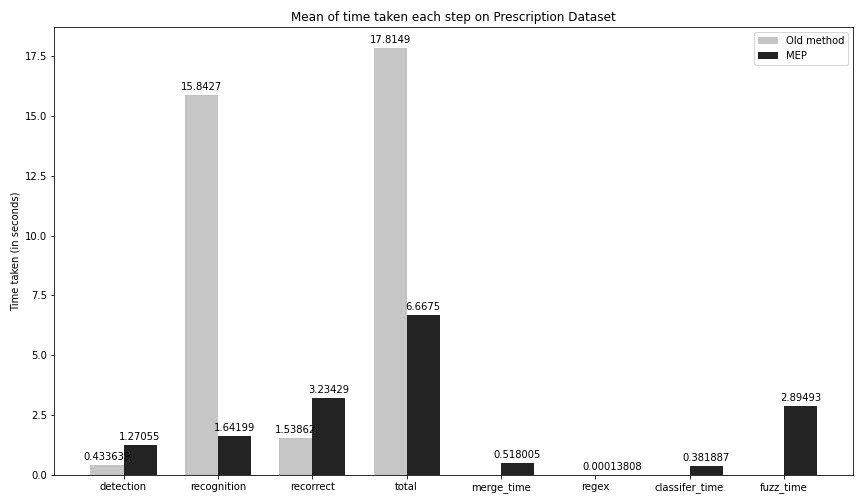
\includegraphics[width=0.7\textwidth]{experiment/charchart1.jpg}
\scalebox{0.55}{%% Creator: Matplotlib, PGF backend
%%
%% To include the figure in your LaTeX document, write
%%   \input{<filename>.pgf}
%%
%% Make sure the required packages are loaded in your preamble
%%   \usepackage{pgf}
%%
%% Also ensure that all the required font packages are loaded; for instance,
%% the lmodern package is sometimes necessary when using math font.
%%   \usepackage{lmodern}
%%
%% Figures using additional raster images can only be included by \input if
%% they are in the same directory as the main LaTeX file. For loading figures
%% from other directories you can use the `import` package
%%   \usepackage{import}
%%
%% and then include the figures with
%%   \import{<path to file>}{<filename>.pgf}
%%
%% Matplotlib used the following preamble
%%
\begingroup%
\makeatletter%
\begin{pgfpicture}%
\pgfpathrectangle{\pgfpointorigin}{\pgfqpoint{9.000000in}{5.000000in}}%
\pgfusepath{use as bounding box, clip}%
\begin{pgfscope}%
\pgfsetbuttcap%
\pgfsetmiterjoin%
\pgfsetlinewidth{0.000000pt}%
\definecolor{currentstroke}{rgb}{1.000000,1.000000,1.000000}%
\pgfsetstrokecolor{currentstroke}%
\pgfsetstrokeopacity{0.000000}%
\pgfsetdash{}{0pt}%
\pgfpathmoveto{\pgfqpoint{0.000000in}{0.000000in}}%
\pgfpathlineto{\pgfqpoint{9.000000in}{0.000000in}}%
\pgfpathlineto{\pgfqpoint{9.000000in}{5.000000in}}%
\pgfpathlineto{\pgfqpoint{0.000000in}{5.000000in}}%
\pgfpathlineto{\pgfqpoint{0.000000in}{0.000000in}}%
\pgfpathclose%
\pgfusepath{}%
\end{pgfscope}%
\begin{pgfscope}%
\pgfsetbuttcap%
\pgfsetmiterjoin%
\definecolor{currentfill}{rgb}{1.000000,1.000000,1.000000}%
\pgfsetfillcolor{currentfill}%
\pgfsetlinewidth{0.000000pt}%
\definecolor{currentstroke}{rgb}{0.000000,0.000000,0.000000}%
\pgfsetstrokecolor{currentstroke}%
\pgfsetstrokeopacity{0.000000}%
\pgfsetdash{}{0pt}%
\pgfpathmoveto{\pgfqpoint{0.516436in}{0.264771in}}%
\pgfpathlineto{\pgfqpoint{8.887500in}{0.264771in}}%
\pgfpathlineto{\pgfqpoint{8.887500in}{4.750662in}}%
\pgfpathlineto{\pgfqpoint{0.516436in}{4.750662in}}%
\pgfpathlineto{\pgfqpoint{0.516436in}{0.264771in}}%
\pgfpathclose%
\pgfusepath{fill}%
\end{pgfscope}%
\begin{pgfscope}%
\pgfpathrectangle{\pgfqpoint{0.516436in}{0.264771in}}{\pgfqpoint{8.371064in}{4.485891in}}%
\pgfusepath{clip}%
\pgfsetbuttcap%
\pgfsetmiterjoin%
\definecolor{currentfill}{rgb}{0.121569,0.466667,0.705882}%
\pgfsetfillcolor{currentfill}%
\pgfsetlinewidth{0.000000pt}%
\definecolor{currentstroke}{rgb}{0.000000,0.000000,0.000000}%
\pgfsetstrokecolor{currentstroke}%
\pgfsetstrokeopacity{0.000000}%
\pgfsetdash{}{0pt}%
\pgfpathmoveto{\pgfqpoint{0.896939in}{0.264771in}}%
\pgfpathlineto{\pgfqpoint{1.242850in}{0.264771in}}%
\pgfpathlineto{\pgfqpoint{1.242850in}{0.368763in}}%
\pgfpathlineto{\pgfqpoint{0.896939in}{0.368763in}}%
\pgfpathlineto{\pgfqpoint{0.896939in}{0.264771in}}%
\pgfpathclose%
\pgfusepath{fill}%
\end{pgfscope}%
\begin{pgfscope}%
\pgfpathrectangle{\pgfqpoint{0.516436in}{0.264771in}}{\pgfqpoint{8.371064in}{4.485891in}}%
\pgfusepath{clip}%
\pgfsetbuttcap%
\pgfsetmiterjoin%
\definecolor{currentfill}{rgb}{0.121569,0.466667,0.705882}%
\pgfsetfillcolor{currentfill}%
\pgfsetlinewidth{0.000000pt}%
\definecolor{currentstroke}{rgb}{0.000000,0.000000,0.000000}%
\pgfsetstrokecolor{currentstroke}%
\pgfsetstrokeopacity{0.000000}%
\pgfsetdash{}{0pt}%
\pgfpathmoveto{\pgfqpoint{1.885258in}{0.264771in}}%
\pgfpathlineto{\pgfqpoint{2.231170in}{0.264771in}}%
\pgfpathlineto{\pgfqpoint{2.231170in}{4.064071in}}%
\pgfpathlineto{\pgfqpoint{1.885258in}{4.064071in}}%
\pgfpathlineto{\pgfqpoint{1.885258in}{0.264771in}}%
\pgfpathclose%
\pgfusepath{fill}%
\end{pgfscope}%
\begin{pgfscope}%
\pgfpathrectangle{\pgfqpoint{0.516436in}{0.264771in}}{\pgfqpoint{8.371064in}{4.485891in}}%
\pgfusepath{clip}%
\pgfsetbuttcap%
\pgfsetmiterjoin%
\definecolor{currentfill}{rgb}{0.121569,0.466667,0.705882}%
\pgfsetfillcolor{currentfill}%
\pgfsetlinewidth{0.000000pt}%
\definecolor{currentstroke}{rgb}{0.000000,0.000000,0.000000}%
\pgfsetstrokecolor{currentstroke}%
\pgfsetstrokeopacity{0.000000}%
\pgfsetdash{}{0pt}%
\pgfpathmoveto{\pgfqpoint{2.873577in}{0.264771in}}%
\pgfpathlineto{\pgfqpoint{3.219489in}{0.264771in}}%
\pgfpathlineto{\pgfqpoint{3.219489in}{0.633754in}}%
\pgfpathlineto{\pgfqpoint{2.873577in}{0.633754in}}%
\pgfpathlineto{\pgfqpoint{2.873577in}{0.264771in}}%
\pgfpathclose%
\pgfusepath{fill}%
\end{pgfscope}%
\begin{pgfscope}%
\pgfpathrectangle{\pgfqpoint{0.516436in}{0.264771in}}{\pgfqpoint{8.371064in}{4.485891in}}%
\pgfusepath{clip}%
\pgfsetbuttcap%
\pgfsetmiterjoin%
\definecolor{currentfill}{rgb}{0.121569,0.466667,0.705882}%
\pgfsetfillcolor{currentfill}%
\pgfsetlinewidth{0.000000pt}%
\definecolor{currentstroke}{rgb}{0.000000,0.000000,0.000000}%
\pgfsetstrokecolor{currentstroke}%
\pgfsetstrokeopacity{0.000000}%
\pgfsetdash{}{0pt}%
\pgfpathmoveto{\pgfqpoint{3.861896in}{0.264771in}}%
\pgfpathlineto{\pgfqpoint{4.207808in}{0.264771in}}%
\pgfpathlineto{\pgfqpoint{4.207808in}{4.537048in}}%
\pgfpathlineto{\pgfqpoint{3.861896in}{4.537048in}}%
\pgfpathlineto{\pgfqpoint{3.861896in}{0.264771in}}%
\pgfpathclose%
\pgfusepath{fill}%
\end{pgfscope}%
\begin{pgfscope}%
\pgfpathrectangle{\pgfqpoint{0.516436in}{0.264771in}}{\pgfqpoint{8.371064in}{4.485891in}}%
\pgfusepath{clip}%
\pgfsetbuttcap%
\pgfsetmiterjoin%
\definecolor{currentfill}{rgb}{1.000000,0.498039,0.054902}%
\pgfsetfillcolor{currentfill}%
\pgfsetlinewidth{0.000000pt}%
\definecolor{currentstroke}{rgb}{0.000000,0.000000,0.000000}%
\pgfsetstrokecolor{currentstroke}%
\pgfsetstrokeopacity{0.000000}%
\pgfsetdash{}{0pt}%
\pgfpathmoveto{\pgfqpoint{1.242850in}{0.264771in}}%
\pgfpathlineto{\pgfqpoint{1.588762in}{0.264771in}}%
\pgfpathlineto{\pgfqpoint{1.588762in}{0.569467in}}%
\pgfpathlineto{\pgfqpoint{1.242850in}{0.569467in}}%
\pgfpathlineto{\pgfqpoint{1.242850in}{0.264771in}}%
\pgfpathclose%
\pgfusepath{fill}%
\end{pgfscope}%
\begin{pgfscope}%
\pgfpathrectangle{\pgfqpoint{0.516436in}{0.264771in}}{\pgfqpoint{8.371064in}{4.485891in}}%
\pgfusepath{clip}%
\pgfsetbuttcap%
\pgfsetmiterjoin%
\definecolor{currentfill}{rgb}{1.000000,0.498039,0.054902}%
\pgfsetfillcolor{currentfill}%
\pgfsetlinewidth{0.000000pt}%
\definecolor{currentstroke}{rgb}{0.000000,0.000000,0.000000}%
\pgfsetstrokecolor{currentstroke}%
\pgfsetstrokeopacity{0.000000}%
\pgfsetdash{}{0pt}%
\pgfpathmoveto{\pgfqpoint{2.231170in}{0.264771in}}%
\pgfpathlineto{\pgfqpoint{2.577081in}{0.264771in}}%
\pgfpathlineto{\pgfqpoint{2.577081in}{0.658542in}}%
\pgfpathlineto{\pgfqpoint{2.231170in}{0.658542in}}%
\pgfpathlineto{\pgfqpoint{2.231170in}{0.264771in}}%
\pgfpathclose%
\pgfusepath{fill}%
\end{pgfscope}%
\begin{pgfscope}%
\pgfpathrectangle{\pgfqpoint{0.516436in}{0.264771in}}{\pgfqpoint{8.371064in}{4.485891in}}%
\pgfusepath{clip}%
\pgfsetbuttcap%
\pgfsetmiterjoin%
\definecolor{currentfill}{rgb}{1.000000,0.498039,0.054902}%
\pgfsetfillcolor{currentfill}%
\pgfsetlinewidth{0.000000pt}%
\definecolor{currentstroke}{rgb}{0.000000,0.000000,0.000000}%
\pgfsetstrokecolor{currentstroke}%
\pgfsetstrokeopacity{0.000000}%
\pgfsetdash{}{0pt}%
\pgfpathmoveto{\pgfqpoint{3.219489in}{0.264771in}}%
\pgfpathlineto{\pgfqpoint{3.565401in}{0.264771in}}%
\pgfpathlineto{\pgfqpoint{3.565401in}{1.040398in}}%
\pgfpathlineto{\pgfqpoint{3.219489in}{1.040398in}}%
\pgfpathlineto{\pgfqpoint{3.219489in}{0.264771in}}%
\pgfpathclose%
\pgfusepath{fill}%
\end{pgfscope}%
\begin{pgfscope}%
\pgfpathrectangle{\pgfqpoint{0.516436in}{0.264771in}}{\pgfqpoint{8.371064in}{4.485891in}}%
\pgfusepath{clip}%
\pgfsetbuttcap%
\pgfsetmiterjoin%
\definecolor{currentfill}{rgb}{1.000000,0.498039,0.054902}%
\pgfsetfillcolor{currentfill}%
\pgfsetlinewidth{0.000000pt}%
\definecolor{currentstroke}{rgb}{0.000000,0.000000,0.000000}%
\pgfsetstrokecolor{currentstroke}%
\pgfsetstrokeopacity{0.000000}%
\pgfsetdash{}{0pt}%
\pgfpathmoveto{\pgfqpoint{4.207808in}{0.264771in}}%
\pgfpathlineto{\pgfqpoint{4.553720in}{0.264771in}}%
\pgfpathlineto{\pgfqpoint{4.553720in}{1.863732in}}%
\pgfpathlineto{\pgfqpoint{4.207808in}{1.863732in}}%
\pgfpathlineto{\pgfqpoint{4.207808in}{0.264771in}}%
\pgfpathclose%
\pgfusepath{fill}%
\end{pgfscope}%
\begin{pgfscope}%
\pgfpathrectangle{\pgfqpoint{0.516436in}{0.264771in}}{\pgfqpoint{8.371064in}{4.485891in}}%
\pgfusepath{clip}%
\pgfsetbuttcap%
\pgfsetmiterjoin%
\definecolor{currentfill}{rgb}{1.000000,0.498039,0.054902}%
\pgfsetfillcolor{currentfill}%
\pgfsetlinewidth{0.000000pt}%
\definecolor{currentstroke}{rgb}{0.000000,0.000000,0.000000}%
\pgfsetstrokecolor{currentstroke}%
\pgfsetstrokeopacity{0.000000}%
\pgfsetdash{}{0pt}%
\pgfpathmoveto{\pgfqpoint{5.196128in}{0.264771in}}%
\pgfpathlineto{\pgfqpoint{5.542039in}{0.264771in}}%
\pgfpathlineto{\pgfqpoint{5.542039in}{0.388995in}}%
\pgfpathlineto{\pgfqpoint{5.196128in}{0.388995in}}%
\pgfpathlineto{\pgfqpoint{5.196128in}{0.264771in}}%
\pgfpathclose%
\pgfusepath{fill}%
\end{pgfscope}%
\begin{pgfscope}%
\pgfpathrectangle{\pgfqpoint{0.516436in}{0.264771in}}{\pgfqpoint{8.371064in}{4.485891in}}%
\pgfusepath{clip}%
\pgfsetbuttcap%
\pgfsetmiterjoin%
\definecolor{currentfill}{rgb}{1.000000,0.498039,0.054902}%
\pgfsetfillcolor{currentfill}%
\pgfsetlinewidth{0.000000pt}%
\definecolor{currentstroke}{rgb}{0.000000,0.000000,0.000000}%
\pgfsetstrokecolor{currentstroke}%
\pgfsetstrokeopacity{0.000000}%
\pgfsetdash{}{0pt}%
\pgfpathmoveto{\pgfqpoint{6.184447in}{0.264771in}}%
\pgfpathlineto{\pgfqpoint{6.530359in}{0.264771in}}%
\pgfpathlineto{\pgfqpoint{6.530359in}{0.264804in}}%
\pgfpathlineto{\pgfqpoint{6.184447in}{0.264804in}}%
\pgfpathlineto{\pgfqpoint{6.184447in}{0.264771in}}%
\pgfpathclose%
\pgfusepath{fill}%
\end{pgfscope}%
\begin{pgfscope}%
\pgfpathrectangle{\pgfqpoint{0.516436in}{0.264771in}}{\pgfqpoint{8.371064in}{4.485891in}}%
\pgfusepath{clip}%
\pgfsetbuttcap%
\pgfsetmiterjoin%
\definecolor{currentfill}{rgb}{1.000000,0.498039,0.054902}%
\pgfsetfillcolor{currentfill}%
\pgfsetlinewidth{0.000000pt}%
\definecolor{currentstroke}{rgb}{0.000000,0.000000,0.000000}%
\pgfsetstrokecolor{currentstroke}%
\pgfsetstrokeopacity{0.000000}%
\pgfsetdash{}{0pt}%
\pgfpathmoveto{\pgfqpoint{7.172766in}{0.264771in}}%
\pgfpathlineto{\pgfqpoint{7.518678in}{0.264771in}}%
\pgfpathlineto{\pgfqpoint{7.518678in}{0.356353in}}%
\pgfpathlineto{\pgfqpoint{7.172766in}{0.356353in}}%
\pgfpathlineto{\pgfqpoint{7.172766in}{0.264771in}}%
\pgfpathclose%
\pgfusepath{fill}%
\end{pgfscope}%
\begin{pgfscope}%
\pgfpathrectangle{\pgfqpoint{0.516436in}{0.264771in}}{\pgfqpoint{8.371064in}{4.485891in}}%
\pgfusepath{clip}%
\pgfsetbuttcap%
\pgfsetmiterjoin%
\definecolor{currentfill}{rgb}{1.000000,0.498039,0.054902}%
\pgfsetfillcolor{currentfill}%
\pgfsetlinewidth{0.000000pt}%
\definecolor{currentstroke}{rgb}{0.000000,0.000000,0.000000}%
\pgfsetstrokecolor{currentstroke}%
\pgfsetstrokeopacity{0.000000}%
\pgfsetdash{}{0pt}%
\pgfpathmoveto{\pgfqpoint{8.161085in}{0.264771in}}%
\pgfpathlineto{\pgfqpoint{8.506997in}{0.264771in}}%
\pgfpathlineto{\pgfqpoint{8.506997in}{0.959016in}}%
\pgfpathlineto{\pgfqpoint{8.161085in}{0.959016in}}%
\pgfpathlineto{\pgfqpoint{8.161085in}{0.264771in}}%
\pgfpathclose%
\pgfusepath{fill}%
\end{pgfscope}%
\begin{pgfscope}%
\pgfsetbuttcap%
\pgfsetroundjoin%
\definecolor{currentfill}{rgb}{0.000000,0.000000,0.000000}%
\pgfsetfillcolor{currentfill}%
\pgfsetlinewidth{0.803000pt}%
\definecolor{currentstroke}{rgb}{0.000000,0.000000,0.000000}%
\pgfsetstrokecolor{currentstroke}%
\pgfsetdash{}{0pt}%
\pgfsys@defobject{currentmarker}{\pgfqpoint{0.000000in}{-0.048611in}}{\pgfqpoint{0.000000in}{0.000000in}}{%
\pgfpathmoveto{\pgfqpoint{0.000000in}{0.000000in}}%
\pgfpathlineto{\pgfqpoint{0.000000in}{-0.048611in}}%
\pgfusepath{stroke,fill}%
}%
\begin{pgfscope}%
\pgfsys@transformshift{1.242850in}{0.264771in}%
\pgfsys@useobject{currentmarker}{}%
\end{pgfscope}%
\end{pgfscope}%
\begin{pgfscope}%
\definecolor{textcolor}{rgb}{0.000000,0.000000,0.000000}%
\pgfsetstrokecolor{textcolor}%
\pgfsetfillcolor{textcolor}%
\pgftext[x=1.242850in,y=0.167548in,,top]{\color{textcolor}\rmfamily\fontsize{10.000000}{12.000000}\selectfont detection}%
\end{pgfscope}%
\begin{pgfscope}%
\pgfsetbuttcap%
\pgfsetroundjoin%
\definecolor{currentfill}{rgb}{0.000000,0.000000,0.000000}%
\pgfsetfillcolor{currentfill}%
\pgfsetlinewidth{0.803000pt}%
\definecolor{currentstroke}{rgb}{0.000000,0.000000,0.000000}%
\pgfsetstrokecolor{currentstroke}%
\pgfsetdash{}{0pt}%
\pgfsys@defobject{currentmarker}{\pgfqpoint{0.000000in}{-0.048611in}}{\pgfqpoint{0.000000in}{0.000000in}}{%
\pgfpathmoveto{\pgfqpoint{0.000000in}{0.000000in}}%
\pgfpathlineto{\pgfqpoint{0.000000in}{-0.048611in}}%
\pgfusepath{stroke,fill}%
}%
\begin{pgfscope}%
\pgfsys@transformshift{2.231170in}{0.264771in}%
\pgfsys@useobject{currentmarker}{}%
\end{pgfscope}%
\end{pgfscope}%
\begin{pgfscope}%
\definecolor{textcolor}{rgb}{0.000000,0.000000,0.000000}%
\pgfsetstrokecolor{textcolor}%
\pgfsetfillcolor{textcolor}%
\pgftext[x=2.231170in,y=0.167548in,,top]{\color{textcolor}\rmfamily\fontsize{10.000000}{12.000000}\selectfont recognition}%
\end{pgfscope}%
\begin{pgfscope}%
\pgfsetbuttcap%
\pgfsetroundjoin%
\definecolor{currentfill}{rgb}{0.000000,0.000000,0.000000}%
\pgfsetfillcolor{currentfill}%
\pgfsetlinewidth{0.803000pt}%
\definecolor{currentstroke}{rgb}{0.000000,0.000000,0.000000}%
\pgfsetstrokecolor{currentstroke}%
\pgfsetdash{}{0pt}%
\pgfsys@defobject{currentmarker}{\pgfqpoint{0.000000in}{-0.048611in}}{\pgfqpoint{0.000000in}{0.000000in}}{%
\pgfpathmoveto{\pgfqpoint{0.000000in}{0.000000in}}%
\pgfpathlineto{\pgfqpoint{0.000000in}{-0.048611in}}%
\pgfusepath{stroke,fill}%
}%
\begin{pgfscope}%
\pgfsys@transformshift{3.219489in}{0.264771in}%
\pgfsys@useobject{currentmarker}{}%
\end{pgfscope}%
\end{pgfscope}%
\begin{pgfscope}%
\definecolor{textcolor}{rgb}{0.000000,0.000000,0.000000}%
\pgfsetstrokecolor{textcolor}%
\pgfsetfillcolor{textcolor}%
\pgftext[x=3.219489in,y=0.167548in,,top]{\color{textcolor}\rmfamily\fontsize{10.000000}{12.000000}\selectfont recorrect}%
\end{pgfscope}%
\begin{pgfscope}%
\pgfsetbuttcap%
\pgfsetroundjoin%
\definecolor{currentfill}{rgb}{0.000000,0.000000,0.000000}%
\pgfsetfillcolor{currentfill}%
\pgfsetlinewidth{0.803000pt}%
\definecolor{currentstroke}{rgb}{0.000000,0.000000,0.000000}%
\pgfsetstrokecolor{currentstroke}%
\pgfsetdash{}{0pt}%
\pgfsys@defobject{currentmarker}{\pgfqpoint{0.000000in}{-0.048611in}}{\pgfqpoint{0.000000in}{0.000000in}}{%
\pgfpathmoveto{\pgfqpoint{0.000000in}{0.000000in}}%
\pgfpathlineto{\pgfqpoint{0.000000in}{-0.048611in}}%
\pgfusepath{stroke,fill}%
}%
\begin{pgfscope}%
\pgfsys@transformshift{4.207808in}{0.264771in}%
\pgfsys@useobject{currentmarker}{}%
\end{pgfscope}%
\end{pgfscope}%
\begin{pgfscope}%
\definecolor{textcolor}{rgb}{0.000000,0.000000,0.000000}%
\pgfsetstrokecolor{textcolor}%
\pgfsetfillcolor{textcolor}%
\pgftext[x=4.207808in,y=0.167548in,,top]{\color{textcolor}\rmfamily\fontsize{10.000000}{12.000000}\selectfont total}%
\end{pgfscope}%
\begin{pgfscope}%
\pgfsetbuttcap%
\pgfsetroundjoin%
\definecolor{currentfill}{rgb}{0.000000,0.000000,0.000000}%
\pgfsetfillcolor{currentfill}%
\pgfsetlinewidth{0.803000pt}%
\definecolor{currentstroke}{rgb}{0.000000,0.000000,0.000000}%
\pgfsetstrokecolor{currentstroke}%
\pgfsetdash{}{0pt}%
\pgfsys@defobject{currentmarker}{\pgfqpoint{0.000000in}{-0.048611in}}{\pgfqpoint{0.000000in}{0.000000in}}{%
\pgfpathmoveto{\pgfqpoint{0.000000in}{0.000000in}}%
\pgfpathlineto{\pgfqpoint{0.000000in}{-0.048611in}}%
\pgfusepath{stroke,fill}%
}%
\begin{pgfscope}%
\pgfsys@transformshift{5.196128in}{0.264771in}%
\pgfsys@useobject{currentmarker}{}%
\end{pgfscope}%
\end{pgfscope}%
\begin{pgfscope}%
\definecolor{textcolor}{rgb}{0.000000,0.000000,0.000000}%
\pgfsetstrokecolor{textcolor}%
\pgfsetfillcolor{textcolor}%
\pgftext[x=5.196128in,y=0.167548in,,top]{\color{textcolor}\rmfamily\fontsize{10.000000}{12.000000}\selectfont merge\_time}%
\end{pgfscope}%
\begin{pgfscope}%
\pgfsetbuttcap%
\pgfsetroundjoin%
\definecolor{currentfill}{rgb}{0.000000,0.000000,0.000000}%
\pgfsetfillcolor{currentfill}%
\pgfsetlinewidth{0.803000pt}%
\definecolor{currentstroke}{rgb}{0.000000,0.000000,0.000000}%
\pgfsetstrokecolor{currentstroke}%
\pgfsetdash{}{0pt}%
\pgfsys@defobject{currentmarker}{\pgfqpoint{0.000000in}{-0.048611in}}{\pgfqpoint{0.000000in}{0.000000in}}{%
\pgfpathmoveto{\pgfqpoint{0.000000in}{0.000000in}}%
\pgfpathlineto{\pgfqpoint{0.000000in}{-0.048611in}}%
\pgfusepath{stroke,fill}%
}%
\begin{pgfscope}%
\pgfsys@transformshift{6.184447in}{0.264771in}%
\pgfsys@useobject{currentmarker}{}%
\end{pgfscope}%
\end{pgfscope}%
\begin{pgfscope}%
\definecolor{textcolor}{rgb}{0.000000,0.000000,0.000000}%
\pgfsetstrokecolor{textcolor}%
\pgfsetfillcolor{textcolor}%
\pgftext[x=6.184447in,y=0.167548in,,top]{\color{textcolor}\rmfamily\fontsize{10.000000}{12.000000}\selectfont regex}%
\end{pgfscope}%
\begin{pgfscope}%
\pgfsetbuttcap%
\pgfsetroundjoin%
\definecolor{currentfill}{rgb}{0.000000,0.000000,0.000000}%
\pgfsetfillcolor{currentfill}%
\pgfsetlinewidth{0.803000pt}%
\definecolor{currentstroke}{rgb}{0.000000,0.000000,0.000000}%
\pgfsetstrokecolor{currentstroke}%
\pgfsetdash{}{0pt}%
\pgfsys@defobject{currentmarker}{\pgfqpoint{0.000000in}{-0.048611in}}{\pgfqpoint{0.000000in}{0.000000in}}{%
\pgfpathmoveto{\pgfqpoint{0.000000in}{0.000000in}}%
\pgfpathlineto{\pgfqpoint{0.000000in}{-0.048611in}}%
\pgfusepath{stroke,fill}%
}%
\begin{pgfscope}%
\pgfsys@transformshift{7.172766in}{0.264771in}%
\pgfsys@useobject{currentmarker}{}%
\end{pgfscope}%
\end{pgfscope}%
\begin{pgfscope}%
\definecolor{textcolor}{rgb}{0.000000,0.000000,0.000000}%
\pgfsetstrokecolor{textcolor}%
\pgfsetfillcolor{textcolor}%
\pgftext[x=7.172766in,y=0.167548in,,top]{\color{textcolor}\rmfamily\fontsize{10.000000}{12.000000}\selectfont classifer\_time}%
\end{pgfscope}%
\begin{pgfscope}%
\pgfsetbuttcap%
\pgfsetroundjoin%
\definecolor{currentfill}{rgb}{0.000000,0.000000,0.000000}%
\pgfsetfillcolor{currentfill}%
\pgfsetlinewidth{0.803000pt}%
\definecolor{currentstroke}{rgb}{0.000000,0.000000,0.000000}%
\pgfsetstrokecolor{currentstroke}%
\pgfsetdash{}{0pt}%
\pgfsys@defobject{currentmarker}{\pgfqpoint{0.000000in}{-0.048611in}}{\pgfqpoint{0.000000in}{0.000000in}}{%
\pgfpathmoveto{\pgfqpoint{0.000000in}{0.000000in}}%
\pgfpathlineto{\pgfqpoint{0.000000in}{-0.048611in}}%
\pgfusepath{stroke,fill}%
}%
\begin{pgfscope}%
\pgfsys@transformshift{8.161085in}{0.264771in}%
\pgfsys@useobject{currentmarker}{}%
\end{pgfscope}%
\end{pgfscope}%
\begin{pgfscope}%
\definecolor{textcolor}{rgb}{0.000000,0.000000,0.000000}%
\pgfsetstrokecolor{textcolor}%
\pgfsetfillcolor{textcolor}%
\pgftext[x=8.161085in,y=0.167548in,,top]{\color{textcolor}\rmfamily\fontsize{10.000000}{12.000000}\selectfont fuzz\_time}%
\end{pgfscope}%
\begin{pgfscope}%
\pgfsetbuttcap%
\pgfsetroundjoin%
\definecolor{currentfill}{rgb}{0.000000,0.000000,0.000000}%
\pgfsetfillcolor{currentfill}%
\pgfsetlinewidth{0.803000pt}%
\definecolor{currentstroke}{rgb}{0.000000,0.000000,0.000000}%
\pgfsetstrokecolor{currentstroke}%
\pgfsetdash{}{0pt}%
\pgfsys@defobject{currentmarker}{\pgfqpoint{-0.048611in}{0.000000in}}{\pgfqpoint{-0.000000in}{0.000000in}}{%
\pgfpathmoveto{\pgfqpoint{-0.000000in}{0.000000in}}%
\pgfpathlineto{\pgfqpoint{-0.048611in}{0.000000in}}%
\pgfusepath{stroke,fill}%
}%
\begin{pgfscope}%
\pgfsys@transformshift{0.516436in}{0.264771in}%
\pgfsys@useobject{currentmarker}{}%
\end{pgfscope}%
\end{pgfscope}%
\begin{pgfscope}%
\definecolor{textcolor}{rgb}{0.000000,0.000000,0.000000}%
\pgfsetstrokecolor{textcolor}%
\pgfsetfillcolor{textcolor}%
\pgftext[x=0.241744in, y=0.216545in, left, base]{\color{textcolor}\rmfamily\fontsize{10.000000}{12.000000}\selectfont \(\displaystyle {0.0}\)}%
\end{pgfscope}%
\begin{pgfscope}%
\pgfsetbuttcap%
\pgfsetroundjoin%
\definecolor{currentfill}{rgb}{0.000000,0.000000,0.000000}%
\pgfsetfillcolor{currentfill}%
\pgfsetlinewidth{0.803000pt}%
\definecolor{currentstroke}{rgb}{0.000000,0.000000,0.000000}%
\pgfsetstrokecolor{currentstroke}%
\pgfsetdash{}{0pt}%
\pgfsys@defobject{currentmarker}{\pgfqpoint{-0.048611in}{0.000000in}}{\pgfqpoint{-0.000000in}{0.000000in}}{%
\pgfpathmoveto{\pgfqpoint{-0.000000in}{0.000000in}}%
\pgfpathlineto{\pgfqpoint{-0.048611in}{0.000000in}}%
\pgfusepath{stroke,fill}%
}%
\begin{pgfscope}%
\pgfsys@transformshift{0.516436in}{0.864306in}%
\pgfsys@useobject{currentmarker}{}%
\end{pgfscope}%
\end{pgfscope}%
\begin{pgfscope}%
\definecolor{textcolor}{rgb}{0.000000,0.000000,0.000000}%
\pgfsetstrokecolor{textcolor}%
\pgfsetfillcolor{textcolor}%
\pgftext[x=0.241744in, y=0.816081in, left, base]{\color{textcolor}\rmfamily\fontsize{10.000000}{12.000000}\selectfont \(\displaystyle {2.5}\)}%
\end{pgfscope}%
\begin{pgfscope}%
\pgfsetbuttcap%
\pgfsetroundjoin%
\definecolor{currentfill}{rgb}{0.000000,0.000000,0.000000}%
\pgfsetfillcolor{currentfill}%
\pgfsetlinewidth{0.803000pt}%
\definecolor{currentstroke}{rgb}{0.000000,0.000000,0.000000}%
\pgfsetstrokecolor{currentstroke}%
\pgfsetdash{}{0pt}%
\pgfsys@defobject{currentmarker}{\pgfqpoint{-0.048611in}{0.000000in}}{\pgfqpoint{-0.000000in}{0.000000in}}{%
\pgfpathmoveto{\pgfqpoint{-0.000000in}{0.000000in}}%
\pgfpathlineto{\pgfqpoint{-0.048611in}{0.000000in}}%
\pgfusepath{stroke,fill}%
}%
\begin{pgfscope}%
\pgfsys@transformshift{0.516436in}{1.463842in}%
\pgfsys@useobject{currentmarker}{}%
\end{pgfscope}%
\end{pgfscope}%
\begin{pgfscope}%
\definecolor{textcolor}{rgb}{0.000000,0.000000,0.000000}%
\pgfsetstrokecolor{textcolor}%
\pgfsetfillcolor{textcolor}%
\pgftext[x=0.241744in, y=1.415616in, left, base]{\color{textcolor}\rmfamily\fontsize{10.000000}{12.000000}\selectfont \(\displaystyle {5.0}\)}%
\end{pgfscope}%
\begin{pgfscope}%
\pgfsetbuttcap%
\pgfsetroundjoin%
\definecolor{currentfill}{rgb}{0.000000,0.000000,0.000000}%
\pgfsetfillcolor{currentfill}%
\pgfsetlinewidth{0.803000pt}%
\definecolor{currentstroke}{rgb}{0.000000,0.000000,0.000000}%
\pgfsetstrokecolor{currentstroke}%
\pgfsetdash{}{0pt}%
\pgfsys@defobject{currentmarker}{\pgfqpoint{-0.048611in}{0.000000in}}{\pgfqpoint{-0.000000in}{0.000000in}}{%
\pgfpathmoveto{\pgfqpoint{-0.000000in}{0.000000in}}%
\pgfpathlineto{\pgfqpoint{-0.048611in}{0.000000in}}%
\pgfusepath{stroke,fill}%
}%
\begin{pgfscope}%
\pgfsys@transformshift{0.516436in}{2.063377in}%
\pgfsys@useobject{currentmarker}{}%
\end{pgfscope}%
\end{pgfscope}%
\begin{pgfscope}%
\definecolor{textcolor}{rgb}{0.000000,0.000000,0.000000}%
\pgfsetstrokecolor{textcolor}%
\pgfsetfillcolor{textcolor}%
\pgftext[x=0.241744in, y=2.015152in, left, base]{\color{textcolor}\rmfamily\fontsize{10.000000}{12.000000}\selectfont \(\displaystyle {7.5}\)}%
\end{pgfscope}%
\begin{pgfscope}%
\pgfsetbuttcap%
\pgfsetroundjoin%
\definecolor{currentfill}{rgb}{0.000000,0.000000,0.000000}%
\pgfsetfillcolor{currentfill}%
\pgfsetlinewidth{0.803000pt}%
\definecolor{currentstroke}{rgb}{0.000000,0.000000,0.000000}%
\pgfsetstrokecolor{currentstroke}%
\pgfsetdash{}{0pt}%
\pgfsys@defobject{currentmarker}{\pgfqpoint{-0.048611in}{0.000000in}}{\pgfqpoint{-0.000000in}{0.000000in}}{%
\pgfpathmoveto{\pgfqpoint{-0.000000in}{0.000000in}}%
\pgfpathlineto{\pgfqpoint{-0.048611in}{0.000000in}}%
\pgfusepath{stroke,fill}%
}%
\begin{pgfscope}%
\pgfsys@transformshift{0.516436in}{2.662913in}%
\pgfsys@useobject{currentmarker}{}%
\end{pgfscope}%
\end{pgfscope}%
\begin{pgfscope}%
\definecolor{textcolor}{rgb}{0.000000,0.000000,0.000000}%
\pgfsetstrokecolor{textcolor}%
\pgfsetfillcolor{textcolor}%
\pgftext[x=0.172299in, y=2.614688in, left, base]{\color{textcolor}\rmfamily\fontsize{10.000000}{12.000000}\selectfont \(\displaystyle {10.0}\)}%
\end{pgfscope}%
\begin{pgfscope}%
\pgfsetbuttcap%
\pgfsetroundjoin%
\definecolor{currentfill}{rgb}{0.000000,0.000000,0.000000}%
\pgfsetfillcolor{currentfill}%
\pgfsetlinewidth{0.803000pt}%
\definecolor{currentstroke}{rgb}{0.000000,0.000000,0.000000}%
\pgfsetstrokecolor{currentstroke}%
\pgfsetdash{}{0pt}%
\pgfsys@defobject{currentmarker}{\pgfqpoint{-0.048611in}{0.000000in}}{\pgfqpoint{-0.000000in}{0.000000in}}{%
\pgfpathmoveto{\pgfqpoint{-0.000000in}{0.000000in}}%
\pgfpathlineto{\pgfqpoint{-0.048611in}{0.000000in}}%
\pgfusepath{stroke,fill}%
}%
\begin{pgfscope}%
\pgfsys@transformshift{0.516436in}{3.262448in}%
\pgfsys@useobject{currentmarker}{}%
\end{pgfscope}%
\end{pgfscope}%
\begin{pgfscope}%
\definecolor{textcolor}{rgb}{0.000000,0.000000,0.000000}%
\pgfsetstrokecolor{textcolor}%
\pgfsetfillcolor{textcolor}%
\pgftext[x=0.172299in, y=3.214223in, left, base]{\color{textcolor}\rmfamily\fontsize{10.000000}{12.000000}\selectfont \(\displaystyle {12.5}\)}%
\end{pgfscope}%
\begin{pgfscope}%
\pgfsetbuttcap%
\pgfsetroundjoin%
\definecolor{currentfill}{rgb}{0.000000,0.000000,0.000000}%
\pgfsetfillcolor{currentfill}%
\pgfsetlinewidth{0.803000pt}%
\definecolor{currentstroke}{rgb}{0.000000,0.000000,0.000000}%
\pgfsetstrokecolor{currentstroke}%
\pgfsetdash{}{0pt}%
\pgfsys@defobject{currentmarker}{\pgfqpoint{-0.048611in}{0.000000in}}{\pgfqpoint{-0.000000in}{0.000000in}}{%
\pgfpathmoveto{\pgfqpoint{-0.000000in}{0.000000in}}%
\pgfpathlineto{\pgfqpoint{-0.048611in}{0.000000in}}%
\pgfusepath{stroke,fill}%
}%
\begin{pgfscope}%
\pgfsys@transformshift{0.516436in}{3.861984in}%
\pgfsys@useobject{currentmarker}{}%
\end{pgfscope}%
\end{pgfscope}%
\begin{pgfscope}%
\definecolor{textcolor}{rgb}{0.000000,0.000000,0.000000}%
\pgfsetstrokecolor{textcolor}%
\pgfsetfillcolor{textcolor}%
\pgftext[x=0.172299in, y=3.813759in, left, base]{\color{textcolor}\rmfamily\fontsize{10.000000}{12.000000}\selectfont \(\displaystyle {15.0}\)}%
\end{pgfscope}%
\begin{pgfscope}%
\pgfsetbuttcap%
\pgfsetroundjoin%
\definecolor{currentfill}{rgb}{0.000000,0.000000,0.000000}%
\pgfsetfillcolor{currentfill}%
\pgfsetlinewidth{0.803000pt}%
\definecolor{currentstroke}{rgb}{0.000000,0.000000,0.000000}%
\pgfsetstrokecolor{currentstroke}%
\pgfsetdash{}{0pt}%
\pgfsys@defobject{currentmarker}{\pgfqpoint{-0.048611in}{0.000000in}}{\pgfqpoint{-0.000000in}{0.000000in}}{%
\pgfpathmoveto{\pgfqpoint{-0.000000in}{0.000000in}}%
\pgfpathlineto{\pgfqpoint{-0.048611in}{0.000000in}}%
\pgfusepath{stroke,fill}%
}%
\begin{pgfscope}%
\pgfsys@transformshift{0.516436in}{4.461520in}%
\pgfsys@useobject{currentmarker}{}%
\end{pgfscope}%
\end{pgfscope}%
\begin{pgfscope}%
\definecolor{textcolor}{rgb}{0.000000,0.000000,0.000000}%
\pgfsetstrokecolor{textcolor}%
\pgfsetfillcolor{textcolor}%
\pgftext[x=0.172299in, y=4.413294in, left, base]{\color{textcolor}\rmfamily\fontsize{10.000000}{12.000000}\selectfont \(\displaystyle {17.5}\)}%
\end{pgfscope}%
\begin{pgfscope}%
\definecolor{textcolor}{rgb}{0.000000,0.000000,0.000000}%
\pgfsetstrokecolor{textcolor}%
\pgfsetfillcolor{textcolor}%
\pgftext[x=0.116744in,y=2.507716in,,bottom,rotate=90.000000]{\color{textcolor}\rmfamily\fontsize{10.000000}{12.000000}\selectfont Time taken (in seconds)}%
\end{pgfscope}%
\begin{pgfscope}%
\pgfsetrectcap%
\pgfsetmiterjoin%
\pgfsetlinewidth{0.803000pt}%
\definecolor{currentstroke}{rgb}{0.000000,0.000000,0.000000}%
\pgfsetstrokecolor{currentstroke}%
\pgfsetdash{}{0pt}%
\pgfpathmoveto{\pgfqpoint{0.516436in}{0.264771in}}%
\pgfpathlineto{\pgfqpoint{0.516436in}{4.750662in}}%
\pgfusepath{stroke}%
\end{pgfscope}%
\begin{pgfscope}%
\pgfsetrectcap%
\pgfsetmiterjoin%
\pgfsetlinewidth{0.803000pt}%
\definecolor{currentstroke}{rgb}{0.000000,0.000000,0.000000}%
\pgfsetstrokecolor{currentstroke}%
\pgfsetdash{}{0pt}%
\pgfpathmoveto{\pgfqpoint{8.887500in}{0.264771in}}%
\pgfpathlineto{\pgfqpoint{8.887500in}{4.750662in}}%
\pgfusepath{stroke}%
\end{pgfscope}%
\begin{pgfscope}%
\pgfsetrectcap%
\pgfsetmiterjoin%
\pgfsetlinewidth{0.803000pt}%
\definecolor{currentstroke}{rgb}{0.000000,0.000000,0.000000}%
\pgfsetstrokecolor{currentstroke}%
\pgfsetdash{}{0pt}%
\pgfpathmoveto{\pgfqpoint{0.516436in}{0.264771in}}%
\pgfpathlineto{\pgfqpoint{8.887500in}{0.264771in}}%
\pgfusepath{stroke}%
\end{pgfscope}%
\begin{pgfscope}%
\pgfsetrectcap%
\pgfsetmiterjoin%
\pgfsetlinewidth{0.803000pt}%
\definecolor{currentstroke}{rgb}{0.000000,0.000000,0.000000}%
\pgfsetstrokecolor{currentstroke}%
\pgfsetdash{}{0pt}%
\pgfpathmoveto{\pgfqpoint{0.516436in}{4.750662in}}%
\pgfpathlineto{\pgfqpoint{8.887500in}{4.750662in}}%
\pgfusepath{stroke}%
\end{pgfscope}%
\begin{pgfscope}%
\definecolor{textcolor}{rgb}{0.000000,0.000000,0.000000}%
\pgfsetstrokecolor{textcolor}%
\pgfsetfillcolor{textcolor}%
\pgftext[x=1.069895in,y=0.410430in,,bottom]{\color{textcolor}\rmfamily\fontsize{10.000000}{12.000000}\selectfont 0.433639}%
\end{pgfscope}%
\begin{pgfscope}%
\definecolor{textcolor}{rgb}{0.000000,0.000000,0.000000}%
\pgfsetstrokecolor{textcolor}%
\pgfsetfillcolor{textcolor}%
\pgftext[x=2.058214in,y=4.105738in,,bottom]{\color{textcolor}\rmfamily\fontsize{10.000000}{12.000000}\selectfont 15.8427}%
\end{pgfscope}%
\begin{pgfscope}%
\definecolor{textcolor}{rgb}{0.000000,0.000000,0.000000}%
\pgfsetstrokecolor{textcolor}%
\pgfsetfillcolor{textcolor}%
\pgftext[x=3.046533in,y=0.675421in,,bottom]{\color{textcolor}\rmfamily\fontsize{10.000000}{12.000000}\selectfont 1.53862}%
\end{pgfscope}%
\begin{pgfscope}%
\definecolor{textcolor}{rgb}{0.000000,0.000000,0.000000}%
\pgfsetstrokecolor{textcolor}%
\pgfsetfillcolor{textcolor}%
\pgftext[x=4.034852in,y=4.578714in,,bottom]{\color{textcolor}\rmfamily\fontsize{10.000000}{12.000000}\selectfont 17.8149}%
\end{pgfscope}%
\begin{pgfscope}%
\definecolor{textcolor}{rgb}{0.000000,0.000000,0.000000}%
\pgfsetstrokecolor{textcolor}%
\pgfsetfillcolor{textcolor}%
\pgftext[x=1.415806in,y=0.611134in,,bottom]{\color{textcolor}\rmfamily\fontsize{10.000000}{12.000000}\selectfont 1.27055}%
\end{pgfscope}%
\begin{pgfscope}%
\definecolor{textcolor}{rgb}{0.000000,0.000000,0.000000}%
\pgfsetstrokecolor{textcolor}%
\pgfsetfillcolor{textcolor}%
\pgftext[x=2.404126in,y=0.700209in,,bottom]{\color{textcolor}\rmfamily\fontsize{10.000000}{12.000000}\selectfont 1.64199}%
\end{pgfscope}%
\begin{pgfscope}%
\definecolor{textcolor}{rgb}{0.000000,0.000000,0.000000}%
\pgfsetstrokecolor{textcolor}%
\pgfsetfillcolor{textcolor}%
\pgftext[x=3.392445in,y=1.082065in,,bottom]{\color{textcolor}\rmfamily\fontsize{10.000000}{12.000000}\selectfont 3.23429}%
\end{pgfscope}%
\begin{pgfscope}%
\definecolor{textcolor}{rgb}{0.000000,0.000000,0.000000}%
\pgfsetstrokecolor{textcolor}%
\pgfsetfillcolor{textcolor}%
\pgftext[x=4.380764in,y=1.905398in,,bottom]{\color{textcolor}\rmfamily\fontsize{10.000000}{12.000000}\selectfont 6.6675}%
\end{pgfscope}%
\begin{pgfscope}%
\definecolor{textcolor}{rgb}{0.000000,0.000000,0.000000}%
\pgfsetstrokecolor{textcolor}%
\pgfsetfillcolor{textcolor}%
\pgftext[x=5.369083in,y=0.430662in,,bottom]{\color{textcolor}\rmfamily\fontsize{10.000000}{12.000000}\selectfont 0.518005}%
\end{pgfscope}%
\begin{pgfscope}%
\definecolor{textcolor}{rgb}{0.000000,0.000000,0.000000}%
\pgfsetstrokecolor{textcolor}%
\pgfsetfillcolor{textcolor}%
\pgftext[x=6.357403in,y=0.306470in,,bottom]{\color{textcolor}\rmfamily\fontsize{10.000000}{12.000000}\selectfont 0.00013808}%
\end{pgfscope}%
\begin{pgfscope}%
\definecolor{textcolor}{rgb}{0.000000,0.000000,0.000000}%
\pgfsetstrokecolor{textcolor}%
\pgfsetfillcolor{textcolor}%
\pgftext[x=7.345722in,y=0.398019in,,bottom]{\color{textcolor}\rmfamily\fontsize{10.000000}{12.000000}\selectfont 0.381887}%
\end{pgfscope}%
\begin{pgfscope}%
\definecolor{textcolor}{rgb}{0.000000,0.000000,0.000000}%
\pgfsetstrokecolor{textcolor}%
\pgfsetfillcolor{textcolor}%
\pgftext[x=8.334041in,y=1.000682in,,bottom]{\color{textcolor}\rmfamily\fontsize{10.000000}{12.000000}\selectfont 2.89493}%
\end{pgfscope}%
\begin{pgfscope}%
\definecolor{textcolor}{rgb}{0.000000,0.000000,0.000000}%
\pgfsetstrokecolor{textcolor}%
\pgfsetfillcolor{textcolor}%
\pgftext[x=4.701968in,y=4.833995in,,base]{\color{textcolor}\rmfamily\fontsize{12.000000}{14.400000}\selectfont Mean of time taken each step on Prescription Dataset}%
\end{pgfscope}%
\begin{pgfscope}%
\pgfsetbuttcap%
\pgfsetmiterjoin%
\definecolor{currentfill}{rgb}{1.000000,1.000000,1.000000}%
\pgfsetfillcolor{currentfill}%
\pgfsetfillopacity{0.800000}%
\pgfsetlinewidth{1.003750pt}%
\definecolor{currentstroke}{rgb}{0.800000,0.800000,0.800000}%
\pgfsetstrokecolor{currentstroke}%
\pgfsetstrokeopacity{0.800000}%
\pgfsetdash{}{0pt}%
\pgfpathmoveto{\pgfqpoint{7.450769in}{4.237544in}}%
\pgfpathlineto{\pgfqpoint{8.790278in}{4.237544in}}%
\pgfpathquadraticcurveto{\pgfqpoint{8.818056in}{4.237544in}}{\pgfqpoint{8.818056in}{4.265322in}}%
\pgfpathlineto{\pgfqpoint{8.818056in}{4.653439in}}%
\pgfpathquadraticcurveto{\pgfqpoint{8.818056in}{4.681217in}}{\pgfqpoint{8.790278in}{4.681217in}}%
\pgfpathlineto{\pgfqpoint{7.450769in}{4.681217in}}%
\pgfpathquadraticcurveto{\pgfqpoint{7.422992in}{4.681217in}}{\pgfqpoint{7.422992in}{4.653439in}}%
\pgfpathlineto{\pgfqpoint{7.422992in}{4.265322in}}%
\pgfpathquadraticcurveto{\pgfqpoint{7.422992in}{4.237544in}}{\pgfqpoint{7.450769in}{4.237544in}}%
\pgfpathlineto{\pgfqpoint{7.450769in}{4.237544in}}%
\pgfpathclose%
\pgfusepath{stroke,fill}%
\end{pgfscope}%
\begin{pgfscope}%
\pgfsetbuttcap%
\pgfsetmiterjoin%
\definecolor{currentfill}{rgb}{0.121569,0.466667,0.705882}%
\pgfsetfillcolor{currentfill}%
\pgfsetlinewidth{0.000000pt}%
\definecolor{currentstroke}{rgb}{0.000000,0.000000,0.000000}%
\pgfsetstrokecolor{currentstroke}%
\pgfsetstrokeopacity{0.000000}%
\pgfsetdash{}{0pt}%
\pgfpathmoveto{\pgfqpoint{7.478547in}{4.521495in}}%
\pgfpathlineto{\pgfqpoint{7.756325in}{4.521495in}}%
\pgfpathlineto{\pgfqpoint{7.756325in}{4.618717in}}%
\pgfpathlineto{\pgfqpoint{7.478547in}{4.618717in}}%
\pgfpathlineto{\pgfqpoint{7.478547in}{4.521495in}}%
\pgfpathclose%
\pgfusepath{fill}%
\end{pgfscope}%
\begin{pgfscope}%
\definecolor{textcolor}{rgb}{0.000000,0.000000,0.000000}%
\pgfsetstrokecolor{textcolor}%
\pgfsetfillcolor{textcolor}%
\pgftext[x=7.867436in,y=4.521495in,left,base]{\color{textcolor}\rmfamily\fontsize{10.000000}{12.000000}\selectfont Method in \cite{nguyen2021developing}}%
\end{pgfscope}%
\begin{pgfscope}%
\pgfsetbuttcap%
\pgfsetmiterjoin%
\definecolor{currentfill}{rgb}{1.000000,0.498039,0.054902}%
\pgfsetfillcolor{currentfill}%
\pgfsetlinewidth{0.000000pt}%
\definecolor{currentstroke}{rgb}{0.000000,0.000000,0.000000}%
\pgfsetstrokecolor{currentstroke}%
\pgfsetstrokeopacity{0.000000}%
\pgfsetdash{}{0pt}%
\pgfpathmoveto{\pgfqpoint{7.478547in}{4.320106in}}%
\pgfpathlineto{\pgfqpoint{7.756325in}{4.320106in}}%
\pgfpathlineto{\pgfqpoint{7.756325in}{4.417328in}}%
\pgfpathlineto{\pgfqpoint{7.478547in}{4.417328in}}%
\pgfpathlineto{\pgfqpoint{7.478547in}{4.320106in}}%
\pgfpathclose%
\pgfusepath{fill}%
\end{pgfscope}%
\begin{pgfscope}%
\definecolor{textcolor}{rgb}{0.000000,0.000000,0.000000}%
\pgfsetstrokecolor{textcolor}%
\pgfsetfillcolor{textcolor}%
\pgftext[x=7.867436in,y=4.320106in,left,base]{\color{textcolor}\rmfamily\fontsize{10.000000}{12.000000}\selectfont MEP}%
\end{pgfscope}%
\end{pgfpicture}%
\makeatother%
\endgroup%
}
\caption{Average processing time in stages}\label{fig_barchart}
\end{figure}

In terms of processing time, our model outperforms with the fastest and slowest processing times across the system at 1.38 seconds and 29.65 seconds, respectively, compared to 3.81 seconds and 51.24 seconds of the previous model. Fig.~\ref{fig_barchart} compares the average processing time of each step on the prescription datasets between the two versions. When Tesseract is replaced by VietOCR that speeds up time from 15.84 second to 1.64 seconds in average. This implies the application of the character recognition model depends on the characteristics of the problem being solved. MEP shortens the required time to match a string to a dictionary. Despite having a lexicon that is more than 100 times larger than the prior one, matching time rose by just 1.69 seconds on average when compared to the previous model.

Overall, the upgraded system has shown a significant improvement in all mentioned metrics. Despite some additional intermediate steps before dictionary matching, our total drug name recognition and the average extraction time is 6.67 seconds per prescription, compared to 17.81 seconds average processing times of the old model. That demonstrates the efficiency in terms of time and accuracy that our model achieves on the problem posed.

\section{Conclusion}
We have developed a prescription recognition system called MEP which assists users in accurately understanding the medicines and avoiding potential risks in the treatment process. The system incorporates various state-of-the-art models in the text detection and recognition phase, as well as the Medicine Classification model and Post-OCR approaches. Experimentation exhibits that the model works with high accuracy and requires little time on the given data set of prescriptions. %However, besides that, there are still many things that this model needs to improve, such as accuracy, uptime and format-diverse prescription.

In the future, the model will be enhanced by including the prescription dictionary into the detection and identification process, which reduces the model's operation time and increases its accuracy. Furthermore, we would attempt to detect prescriptions that are fully independent on the pattern, and include tasks such as advising patients to utilize the drug appropriately and reminding them of the time to take medicine. 

%Our technology will provide several benefits in the medical industry, allowing users to swiftly and conveniently acquire the information they require.

\subsubsection{Acknowledgements}
This research is funded by the University of Science, VNU-HCM, Vietnam under grant number CNTT 2021-12 and Advanced Program in Computer Science.

\printbibliography %Prints bibliography
\end{document}


%
% ---- Bibliography ----
%
% BibTeX users should specify bibliography style 'splncs04'.
% References will then be sorted and formatted in the correct style.
%
% \bibliographystyle{splncs04}
% \bibliography{mybibliography}
%
% \begin{thebibliography}{8}
% \bibitem{ref_article1}
% Author, F.: Article title. Journal \textbf{2}(5), 99--110 (2016)

% \bibitem{ref_lncs1}
% Author, F., Author, S.: Title of a proceedings paper. In: Editor,
% F., Editor, S. (eds.) CONFERENCE 2016, LNCS, vol. 9999, pp. 1--13.
% Springer, Heidelberg (2016). \doi{10.10007/1234567890}

% \bibitem{ref_book1}
% Author, F., Author, S., Author, T.: Book title. 2nd edn. Publisher,
% Location (1999)

% \bibitem{ref_proc1}
% Author, A.-B.: Contribution title. In: 9th International Proceedings
% on Proceedings, pp. 1--2. Publisher, Location (2010)

% \bibitem{ref_url1}
% LNCS Homepage, \url{http://www.springer.com/lncs}. Last accessed 4
% Oct 2017
% \end{thebibliography}

